% CVPR 2026 Paper Template — arXiv version
% see https://github.com/cvpr-org/author-kit

\documentclass[10pt,twocolumn,letterpaper]{article}

% Pass options to packages loaded internally by cvpr.sty
\PassOptionsToPackage{table}{xcolor}

%%%%%%%%% PAPER TYPE
% \usepackage{cvpr}              % To produce the CAMERA-READY version
% \usepackage[review]{cvpr}      % To produce the REVIEW version
\usepackage[pagenumbers]{cvpr}   % arXiv version: non-anonymous, with page numbers

% Include additional packages here, before hyperref.
\usepackage{graphicx}
\usepackage{amsmath}
\usepackage{amssymb}
\usepackage{booktabs}
\usepackage{realboxes}
\usepackage[ruled]{algorithm2e}
\renewcommand{\algorithmcfname}{ALGORITHM}
\SetAlFnt{\small}
\SetAlCapFnt{\small}
\SetAlCapNameFnt{\small}
\SetAlCapHSkip{0pt}

\definecolor{cvprblue}{rgb}{0.21,0.49,0.74}
\usepackage[pagebackref,breaklinks,colorlinks,allcolors=cvprblue]{hyperref}

\usepackage[capitalize]{cleveref}
\usepackage{capt-of}   % for \captionof used in the teaser strip
\crefname{section}{Sec.}{Secs.}
\Crefname{section}{Section}{Sections}
\Crefname{table}{Table}{Tables}
\crefname{table}{Tab.}{Tabs.}

% Method name — change once here to update everywhere
\newcommand{\methodname}{SeamGen}

\newcommand{\tightcolorbox}[2]{%
  \begingroup
  \setlength{\fboxsep}{1pt}%
  \colorbox{#1}{#2}%
  \endgroup
}

\definecolor{valueColor}{RGB}{235, 245, 255}
\definecolor{gtColor}{RGB}{255, 245, 235}
\newcommand{\lyt}[1]{\textcolor{blue}{#1}}

%%%%%%%%% PAPER ID  (arXiv: not used for review, keep placeholder)
\def\paperID{0000}
\def\confName{CVPR}
\def\confYear{2026}


\begin{document}

%%%%%%%%% TITLE
\title{\methodname: Artist-Aligned UV Seam Generation via Graph Flow Matching}

%%%%%%%%% AUTHORS - PLEASE FILL IN
% Multi-author, two-institution layout.
% - Use $^{1}$, $^{2}$ superscripts on names to mark affiliation.
% - Corresponding author: add $^{\dagger}$ (or {*}) and explain via \thanks or footnote.
% - Emails: list the ones you want to show; comma-separate.
\author{%
  Hao Xu$^{1}$ \quad
  Yuqing Zhang$^{1}$ \quad
  Yiqian Wu$^{1}$ \quad
  Xueqi Ma$^{2}$ \quad
  Ding Liang$^{2}$ \quad
  Yan-Pei Cao$^{2}$
  \\[0.3em]
  Ying-Tian Liu$^{2}$ \quad
  Xiaogang Jin$^{1}$\thanks{Corresponding author.}
  \\[0.4em]
  $^{1}$State Key Lab of CAD\&CG, Zhejiang University \quad
  $^{2}$VAST
}

\twocolumn[{%
  \begin{@twocolumnfalse}
    \maketitle
    \begin{center}
      \centering
      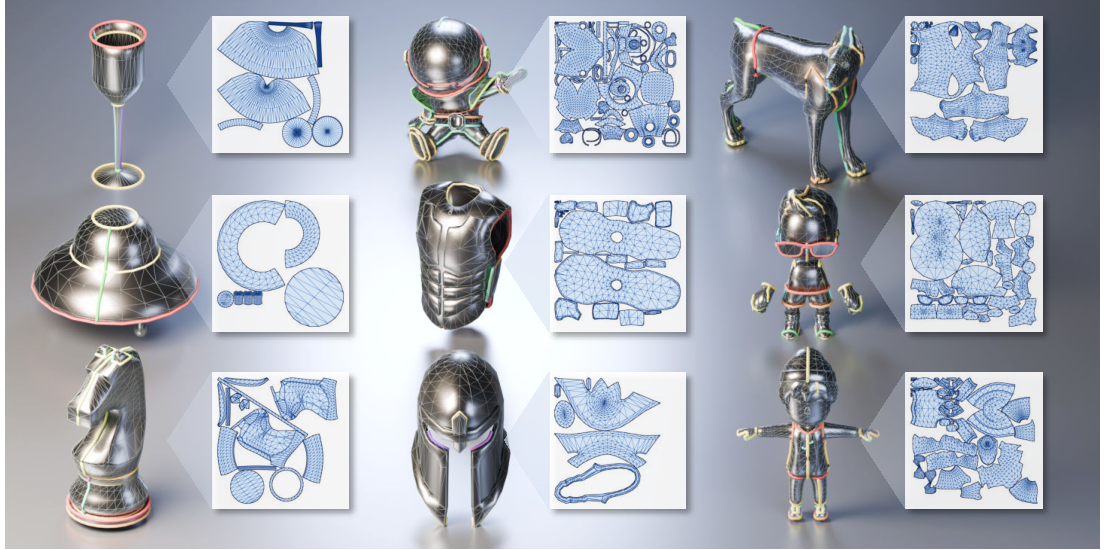
\includegraphics[width=0.99\textwidth]{figures/teaser_new.pdf}
      \captionof{figure}{%
        \textbf{\methodname{} generates UV seams that match artist conventions.}
        Instead of relying on hand-crafted distortion objectives for optimization, \methodname{} models the distribution of artist-authored seam layouts on irregular mesh graphs, generating coherent seam paths and well-structured UV islands that preserve semantic parts, reduce unnecessary fragmentation, place seams away from visually salient regions, and better support texture authoring in practice.%
      }\label{fig:teaser}
    \end{center}
    \vspace{1em}
  \end{@twocolumnfalse}
}]

\begin{abstract}
UV seam placement is a critical yet labor-intensive step in 3D content creation, requiring artists to balance chart shape, seam concealment, and alignment with semantic and geometric features. Existing automatic methods are primarily based on per-object optimization, relying on handcrafted objectives to avoid distortion or on proxies from pretrained models to inject semantic information. However, these strategies are not always well aligned with seams used in industrial production pipelines, often resulting in layouts that deviate from artist-preferred seam patterns and practical production requirements. 
To address these limitations, we propose \textit{\methodname{}}, a generative model for UV seam generation that aligns with artist preferences and production requirements. 
Instead of depending on manually designed objectives and constraints, \methodname{} learns the distribution of per-edge seam labels from a large corpus of existing seam layouts using a flow-matching generative model.
A key challenge is that typical Transformer architectures used in flow matching models are designed for sequential representations, such as point clouds, and cannot naturally account for mesh topology. To enable mesh-native learning, we design a Mesh Transformer backbone that interleaves local graph attention over mesh edges with global self-attention across vertices, capturing both fine-grained geometric cues and long-range topological coherence. 
To further improve inference-time controllability and quality, we exploit the training-free inpainting capability of flow models for both localized seam refinement and constraint-guided seam generation.
Extensive experiments show that by learning priors from professional seam layout data, \methodname{} produces UV layouts that better align with artist-authored preferences and achieve superior perceptual quality compared with distortion-based and semantic-proxy baselines.
\end{abstract}

%%%%%%%%% BODY TEXT
\section{Introduction}
UV unwrapping is an essential step in 3D asset production, enabling textures and material details to be applied through a 2D parameterization of the mesh surface. Its quality depends critically on seam placement, i.e., where the surface is cut before flattening.  
% Manual seam placement remains tedious and expertise-demanding. Desirable seams depend not only on geometric distortion, but also on perceptual visibility, semantic part boundaries, and artist conventions. To reduce this manual effort, existing automatic UV unwrapping methods attempt to determine seams and parameterizations automatically, often through hand-crafted geometric objectives or heuristic chart construction.
Manual seam placement remains tedious and expertise-demanding. Desirable seams depend not only on geometric distortion, but also on perceptual visibility, semantic part boundaries, and artist conventions~\cite{DBLP:conf/visualization/ShefferH02,DBLP:conf/siggrapha/LucquinDB17,wang2025partuv}. To reduce this manual effort, 
%existing 
automatic UV unwrapping methods seek to generate seams and parameterizations automatically, typically by formulating UV unwrapping as a geometry-driven optimization problem.
% This motivates research on automatic UV unwrapping methods. 

% UV unwrapping is a crucial step in 3D asset production, enabling the application of textures and material details through a 2D parameterization of the mesh surface. The quality of this process hinges on seam placement—specifically, where the surface is cut before flattening. Ideal seams are influenced not only by geometric distortion but also by perceptual visibility, semantic part boundaries, and artistic conventions. As a result, automatic UV unwrapping methods have been developed to replace manual seam placement, alleviating the time-consuming and expertise-intensive nature of the task.
 
Most existing approaches are based on per-object optimization with geometric distortion objectives, such as angle or area preservation~\cite{levy2002least, sheffer2005abf, rabinovich2017scalable, li2018optcuts}, while more recent methods, such as PartUV~\cite{wang2025partuv}, additionally incorporate semantic part segmentation as a proxy for structured chart layouts. However, handcrafted objectives and semantic proxies are not always well aligned with the industrial production requirements. 
As a result, layouts produced by current methods often fail to place seams in ways that support practical texture authoring, such as avoiding visually salient regions and preserving texture continuity across important surface areas.
% deviate substantially from those created by professional artists and remain unsuitable for production use. 
%
% In particular, they often fail to place seams in ways that support practical texture authoring.
% , such as avoiding visually salient regions and preserving texture continuity across important surface areas.
For the example of a dog model (see Fig. \ref{fig:artist}), artists typically avoid placing seams on the face. In contrast, methods such as xatlas~\cite{young2019xatlas} and PartUV~\cite{wang2025partuv} often introduce excessive seams in this region to reduce distortion, which disrupts texture continuity and increases the risk of visible artifacts.
%
This can be attributed to the gap between explicit optimization objectives and the complex seam design preferences encountered in real-world settings, where the latter often involve practical, perceptual, semantic, and geometric factors shaped by visual experience and production requirements.
Consequently, per-object optimization is inherently constrained. These observations motivate a data-driven formulation that learns seam placement directly from artist-authored examples. 


\begin{figure}
    \centering
    \vspace{-6mm}
    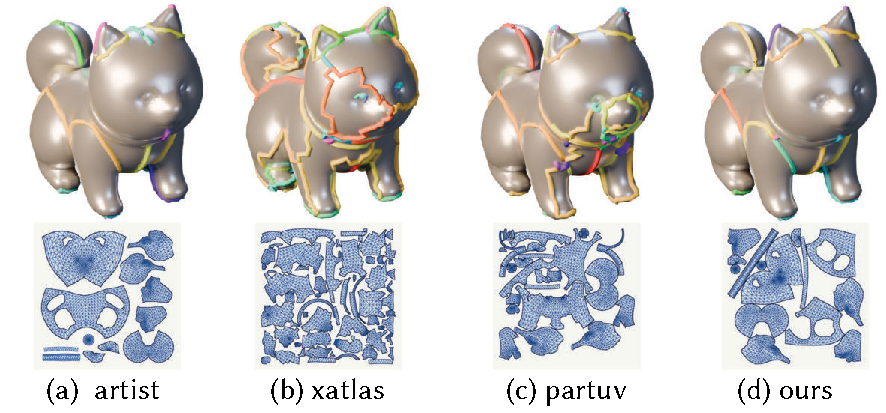
\includegraphics[width=\linewidth]{figures/artist.pdf}
    \caption{
    \textbf{Comparison with artist-authored seam placement.}
    (a) Artist-authored seams avoid salient regions (e.g., the face), favoring inconspicuous boundaries.
    (b-c) Distortion-oriented methods such as xatlas and PartUV produce seam layouts that differ substantially from the artist-authored reference, with seams often appearing in visually important facial regions.
    (d) \methodname{} better matches the artist-authored seam distribution, preserving the face while placing cuts along more natural boundaries.
    }
    \vspace{-6mm}
    \label{fig:artist}
\end{figure}


 

% To this end, we propose \textit{\methodname{}}, which formulates UV seam generation as a distribution-fitting problem on the mesh graph. 
To this end, we propose \textit{\methodname{}}, which formulates surface seam cutting as a conditional generation problem on the mesh graph, learning the distribution of artist-authored seam layouts conditioned on the input geometry.
Seam generation is challenging because seam edges occupy only a small fraction of all mesh edges, yet should still respect geometry, semantics, artist conventions, and topology on irregular mesh connectivity.  
% Instead of independently identifying seams from all edges, we adopt flow matching~\cite{lipman2023flow} as our generative formulation, learning to transform random edge-wise noise into a structured seam probability field. 
Instead of independently identifying seams from all edges, we adopt flow matching~\cite{lipman2023flow} as our generative formulation, learning to transform random edge-wise noise into a coherent binary seam indicator on the mesh graph.
A key challenge is that typical Transformer architectures are designed for sequential modeling and are therefore better suited to representations such as point clouds, without naturally accounting for mesh topology. However, seam decisions depend on both global context, which coordinates cuts into coherent layouts across the entire shape, and local geometric cues, such as dihedral angles and curvature, which determine where seams should be placed in a topology-aware manner.
%
To enable mesh-native learning, we design a Mesh Transformer backbone that interleaves local graph attention over mesh edges with global self-attention across vertices, capturing both fine-grained geometric cues and long-range topological coherence.
% 
% To support localized control, we further exploit the training-free inpainting capability of flow models for conditional seam editing. 
% Given sparse user constraints, such as seam-free regions or prescribed cut edges, we clamp the specified edges during sampling and re-generate the remaining seam layout using the same learned flow model. 
% This allows \methodname{} to complete user-guided layouts while preserving artist-like seam statistics. 
% Beyond manual editing, we instantiate this conditional generation principle as a validity-aware self-refinement procedure. 
% When an initial layout induces an invalid UV atlas, \methodname{} anchors the reliable seams and selectively re-samples the problematic subgraph under these constraints. 
% This inference-time correction improves atlas validity while preserving the global seam organization and artist-authored statistics learned by the model.
To support localized control, we further exploit the learned flow model as a training-free conditional prior. 
Given sparse user constraints, such as seam-free regions or prescribed cut edges, \methodname{} clamps the specified edges during sampling and regenerates the remaining seam layout. 
The same mechanism also enables overlap self-refinement: when an initial layout produces invalid UV overlaps, we fix the reliable seams and resample only the problematic local region. 
This enables constrained editing and inference-time correction without additional training or a separate repair model.
Together, these designs enable \methodname{} to generate seam layouts that better match \textit{artist-authored priors} while remaining robust in practical UV unwrapping scenarios.

In summary, our contributions are as follows:
\begin{itemize}
    % \item We formulate UV seam cutting as mesh-edge seam generation rather than distortion-driven optimization, and propose \methodname{}, the first flow-matching-based framework for learning artist-authored seam layout priors from real-world UV data.
    \item We formulate UV seam cutting as mesh-edge seam generation and propose \methodname{}, the first flow-matching framework that learns artist-authored seam layout priors from real-world UV data.
    \item We develop a mesh-native Mesh Transformer for seam prediction on mesh graphs, and reuse the learned flow model as a training-free conditional prior for constraint-guided completion and overlap self-refinement.
    \item We demonstrate that by learning priors from professional seam  data, \methodname{} produces better artist-aligned UV layouts with superior perceptual quality than baselines.
\end{itemize}


\section{Related Work}

% \subsection{UV Mapping and Seam Placement}

% Surface parameterization, which maps a 3D mesh to a 2D domain, has a long history in computer graphics~\cite{floater2005surface, sheffer2006mesh}. 
% Classical methods include fixed-boundary formulations~\cite{tutte1963draw}, free-boundary and conformal approaches~\cite{levy2002least, sheffer2001parameterization, sheffer2005abf, mullen2008spectral, sawhney2021boundary, ben2009conformal}, and distortion-minimizing or injectivity-preserving optimization methods~\cite{sorkine2007arap, hormann2000mips, rabinovich2017scalable, li2018optcuts, pietroni2010almost, digne2016area, chen2012optimizing}.
% While effective at reducing distortion and enforcing injectivity, these methods are largely driven by handcrafted geometric objectives and do not model the semantic or functional seam-placement priors that artists embed in UV layouts.

% Because parameterization quality depends heavily on how the surface is cut into UV islands, a large body of work has also studied seam placement explicitly.
% Bottom-up methods grow and merge charts under distortion bounds~\cite{julius2005d, sorkine2002bounded, levy2001bounded, sander2003multi, carr2006rectangular}, forming the basis of practical tools such as xatlas~\cite{young2019xatlas} and Blender's Smart UV Project~\cite{blender}, but often produce over-fragmented atlases.
% Other approaches derive cuts from spectral analysis~\cite{zhou2004iso}, geometric feature lines~\cite{zhang2005feature, carlsson2014optimized}, or variational objectives that balance seam complexity and mapping distortion~\cite{liu2007mesh, poranne2017autocuts, sharp2018variational, li2018optcuts}.
% However, these methods remain geometry-driven and do not exploit the rich priors available in artist-authored UV datasets.

% To overcome the limitations of purely geometry-driven methods, recent learning-based approaches have explored data-driven formulations for UV generation and seam prediction. 
% Neural parameterization methods learn continuous surface-to-domain mappings or distortion-aware representations~\cite{groueix2018papier, morreale2021neural, zhao2024flexpara, srinivasan2024nuvo, zhang2024flatten, liu2024dawand}, but do not explicitly model artist-authored seam-layout priors. 
% PartUV~\cite{wang2025partuv} incorporates semantic part cues into chart decomposition by grouping faces according to both distortion and feature similarity, but it still does not explicitly model the distribution of artist-authored seam layouts from data.
% Seamcrafter~\cite{liu2025seamcrafter} addresses this via reinforcement learning to generate seams aligned with artist preferences, and concurrent seam-generation preprints, including SeamGPT~\cite{li2025seamgpt} and MeshTailor~\cite{ma2026meshtailor}, move closer to our setting by learning seams directly from data, but both rely on autoregressive generation. 
% By contrast, our method directly learns a stochastic distribution over artist-authored seam layouts on mesh edges and predicts all seams simultaneously.

% \subsection{Geometry-driven UV Mapping}

% Surface parameterization, which maps a 3D mesh to a 2D domain, has a long history in computer graphics~\cite{floater2005surface, sheffer2006mesh}. 
% Classical methods include fixed-boundary formulations~\cite{tutte1963draw}, free-boundary and conformal approaches~\cite{levy2002least, sheffer2001parameterization, sheffer2005abf, mullen2008spectral, sawhney2021boundary, ben2009conformal}, and distortion-minimizing or injectivity-preserving optimization methods~\cite{sorkine2007arap, hormann2000mips, rabinovich2017scalable, li2018optcuts, pietroni2010almost, digne2016area, chen2012optimizing}.
% These methods remain effective for producing low-distortion and valid parameterizations.
% However, they are primarily driven by handcrafted geometric objectives, such as angle preservation, area preservation, stretch minimization, or injectivity constraints, and therefore do not explicitly model the semantic or functional preferences that artists encode when placing seams.

% Because parameterization quality depends heavily on how the surface is cut into UV islands, a large body of work has also studied seam placement and chart decomposition explicitly.
% Bottom-up methods grow and merge charts under distortion bounds~\cite{julius2005d, sorkine2002bounded, levy2001bounded, sander2003multi, carr2006rectangular}, forming the basis of practical tools such as xatlas~\cite{young2019xatlas} and Blender's Smart UV Project~\cite{blender}.
% These approaches are efficient and widely used, but often produce over-fragmented atlases.
% Other methods derive cuts from spectral analysis~\cite{zhou2004iso}, geometric feature lines~\cite{zhang2005feature, carlsson2014optimized}, or variational objectives that balance seam complexity and mapping distortion~\cite{liu2007mesh, poranne2017autocuts, sharp2018variational, li2018optcuts}.
% Although these methods improve the trade-off between seam length, chart structure, and parameterization distortion, they remain largely geometry-driven and do not exploit the rich priors available in artist-authored UV layouts.

\subsection{Geometry-driven UV Mapping}

Constructing a UV atlas requires determining both how to cut a surface into charts and how to flatten the resulting charts into a 2D domain. 
A long line of work addresses these problems through handcrafted geometric objectives~\cite{floater2005surface, sheffer2006mesh}. 
Classical surface parameterization methods include fixed-boundary formulations~\cite{tutte1963draw}, free-boundary and conformal approaches~\cite{levy2002least, sheffer2001parameterization, sheffer2005abf, mullen2008spectral, sawhney2021boundary, ben2009conformal}, and distortion-minimizing or injectivity-preserving optimization methods~\cite{sorkine2007arap, hormann2000mips, rabinovich2017scalable, li2018optcuts, pietroni2010almost, digne2016area, chen2012optimizing}.
These methods are effective for producing low-distortion and valid parameterizations, but they mainly optimize the geometric quality of the 2D map, such as angle preservation, area preservation, stretch minimization, or injectivity.
Because the choice of cuts strongly affects the parameterization domain and the structure of the resulting UV atlas, many geometry-driven methods also explicitly study seam placement and chart decomposition.
Bottom-up methods grow and merge charts under distortion bounds~\cite{julius2005d, DBLP:conf/visualization/SorkineCGL02, sander2003multi, carr2006rectangular}, forming the basis of practical tools such as xatlas~\cite{young2019xatlas} and Blender's Smart UV Project~\cite{blender}.
Other methods derive cuts from spectral analysis~\cite{zhou2004iso}, geometric feature lines~\cite{zhang2005feature, carlsson2014optimized}, or variational objectives that balance seam complexity and mapping distortion~\cite{liu2007mesh, poranne2017autocuts, sharp2018variational, li2018optcuts}.
However, they remain driven by predefined geometric criteria, rather than the semantic and perceptual preferences reflected in artist-authored UV layouts.


\subsection{Learning-based Surface Parameterization}

Recent work has explored neural formulations for surface parameterization and UV generation.
Neural parameterization methods learn continuous surface-to-domain mappings or distortion-aware representations~\cite{groueix2018papier, morreale2021neural, zhao2024flexpara, srinivasan2024nuvo, zhang2024flatten, liu2024dawand}.
Although these methods use neural networks, they are typically optimized with self-supervised geometric objectives, such as distortion, reconstruction, or injectivity-related losses.
Moreover, they commonly formulate UV generation as a point-wise mapping problem, where surface points or vertices are mapped continuously to 2D coordinates.
This differs from our setting, which focuses on predicting a discrete seam layout on the mesh connectivity and thereby determining a chart decomposition before flattening.
As a result, these methods mainly learn parameterizations or distortion-aware mappings, rather than modeling artist-authored seam distributions.

More recent methods move closer to data-driven UV decomposition.
PartUV~\cite{wang2025partuv} incorporates semantic part cues into chart decomposition by grouping faces according to both distortion and feature similarity.
Strips as Tokens~\cite{xu2026strips} introduces an autoregressive mesh generation framework with native UV segmentation, but its UV decomposition is generated as part of mesh generation rather than predicted for an existing input mesh.Concurrent work also explores data-driven seam generation.
SeamGPT~\cite{li2025seamgpt} and MeshTailor~\cite{ma2026meshtailor} learn seam layouts from data, while SeamCrafter~\cite{liu2025seamcrafter} further incorporates reinforcement learning to improve autoregressive seam generation.
Our method instead formulates seam cutting as generation on the mesh edge graph, using flow matching to jointly produce the full seam layout for a given input mesh.

% More recent methods move closer to seam prediction and chart decomposition.
% PartUV~\cite{wang2025partuv} incorporates semantic part cues into chart decomposition by grouping faces according to both distortion and feature similarity.
% However, it does not directly learn a stochastic distribution over artist-authored seam layouts.
% Seamcrafter~\cite{liu2025seamcrafter} addresses artist-preferred seam generation through reinforcement learning, while concurrent seam-generation preprints, including SeamGPT~\cite{li2025seamgpt} and MeshTailor~\cite{ma2026meshtailor}, learn seams directly from data.
% These methods represent an important step toward data-driven seam generation, but they rely on sequential or autoregressive generation procedures. In contrast, our method directly learns a stochastic distribution over artist-authored seam layouts on mesh edges.
% Given a mesh, it predicts all seam decisions jointly through a flow-matching formulation, enabling non-autoregressive generation of coherent seam layouts that capture both global chart structure and local seam-placement cues.

% \subsection{Generative Models on Meshes}

% Recent progress in generative modeling on meshes has been largely driven by the challenge of representing complex mesh structure in a form amenable to generation. Autoregressive methods tokenize meshes into sequential representations~\cite{nash2020polygen, yan2022shapeformer, chen2024octgpt, siddiqui2024meshgpt, tang2025edgerunner, weng2025scaling, wu2024llamamesh, chen2025meshtron}, progressively improving fidelity and scalability through better tokenization and sequence design. More recent methods reduce the reliance on direct token-by-token generation over native mesh topology: diffusion and flow-based approaches operate on alternative 3D representations~\cite{alliegro2023polydiff, he2025meshcraft, zhao2023michelangelo, liu2024object64, zhang2023shape2vecset}, while TRELLIS~\cite{xiang2025structured,trellis2}, Hunyuan3D~\cite{zhao2025hunyuan3d,hunyuan25}, and TripoSG~\cite{li2025triposg} generate expressive intermediate 3D representations that can be decoded into meshes. Despite their differences in representation and generation mechanism, these methods all aim to synthesize new mesh geometry or topology from scratch. By contrast, our setting assumes a fixed input mesh graph and models a stochastic distribution over binary seam labels on its edges, making our task a mesh analysis problem rather than mesh synthesis.


% \subsection{Generative Models on Meshes}

% Recent progress in generative modeling on meshes has been largely driven by the challenge of representing complex mesh structure in a form amenable to generation. Autoregressive methods tokenize meshes into sequential representations~\cite{nash2020polygen, yan2022shapeformer, chen2024octgpt, siddiqui2024meshgpt, tang2025edgerunner, weng2025scaling, wu2024llamamesh, chen2025meshtron}, progressively improving fidelity and scalability through better tokenization and sequence design. More recent methods reduce the reliance on direct token-by-token generation over native mesh topology: diffusion and flow-based approaches operate on alternative 3D representations~\cite{alliegro2023polydiff, he2025meshcraft, zhao2023michelangelo, liu2024object64, zhang2023shape2vecset}, while TRELLIS~\cite{xiang2025structured,trellis2}, Hunyuan3D~\cite{zhao2025hunyuan3d,hunyuan25}, and TripoSG~\cite{li2025triposg} generate expressive intermediate 3D representations that can be decoded into meshes. Despite their differences in representation and generation mechanism, these methods all aim to synthesize new mesh geometry or topology from scratch. By contrast, our setting assumes a fixed input mesh graph and models a stochastic distribution over binary seam labels on its edges, making our task a mesh analysis problem rather than mesh synthesis.


% \section{Related Work}

% \subsection{UV Mapping and Seam Placement}

% Surface parameterization, which maps a 3D mesh to a 2D domain, has a long history in computer graphics~\cite{floater2005surface, sheffer2006mesh}. 
% Classical methods include fixed-boundary formulations based on Laplacian systems~\cite{tutte1963draw}, free-boundary approaches such as LSCM and ABF/ABF++~\cite{levy2002least, sheffer2001parameterization, sheffer2005abf}, and more recent optimization-based methods such as SLIM and OptCuts~\cite{rabinovich2017scalable, li2018optcuts}. 
% While effective at reducing distortion and enforcing injectivity, these methods are largely driven by handcrafted geometric objectives and do not model the semantic or functional seam-placement priors that artists embed in UV layouts.

% Because parameterization quality depends heavily on how the surface is cut into UV islands, a large body of work has also studied seam placement explicitly. 
% Bottom-up methods grow and merge charts under distortion bounds~\cite{julius2005d, sorkine2002bounded}, forming the basis of practical tools such as xatlas~\cite{young2019xatlas} and Blender's Smart UV Project~\cite{blender}, but often produce over-fragmented atlases. 
% Other approaches derive cuts from spectral analysis, feature lines, or variational objectives that balance seam complexity and mapping distortion~\cite{liu2007mesh, zhang2005feature, poranne2017autocuts, sharp2018variational, li2018optcuts}. 
% However, these methods remain geometry-driven and do not exploit the rich priors available in artist-authored UV datasets.

% To overcome the limitations of purely geometry-driven methods, recent learning-based approaches have explored data-driven formulations for UV generation and seam prediction. 
% Neural parameterization methods such as AtlasNet~\cite{groueix2018papier}, Neural Surface Maps~\cite{morreale2021neural}, Nuvo~\cite{srinivasan2024nuvo}, and FAM~\cite{zhang2024flatten} learn continuous surface-to-domain mappings, but do not explicitly model artist-authored seam-layout priors. 
% PartUV~\cite{wang2025partuv} incorporates semantic part cues into chart decomposition by grouping faces according to both distortion and feature similarity, but it still does not explicitly model the distribution of artist-authored seam layouts from data. 
% Concurrent seam-generation preprints, including SeamGPT~\cite{li2025seamgpt} and MeshTailor~\cite{ma2026meshtailor}, move closer to our setting by learning seams directly from data, but both rely on autoregressive generation. 
% By contrast, our method directly learns a stochastic distribution over artist-authored seam layouts on mesh edges and predicts all seams simultaneously.


% More recent learning-based methods move beyond purely handcrafted geometric optimization, but most still do not explicitly model the distribution of artist-authored UV layouts from data. Neural parameterization approaches such as AtlasNet~\cite{groueix2018papier}, Neural Surface Maps~\cite{morreale2021neural}, and Nuvo~\cite{srinivasan2024nuvo} learn continuous mappings between 3D surfaces and 2D domains, but typically rely on per-shape optimization and are not naturally aligned with standard mesh-based UV pipelines that require explicit edge-level seams and discrete UV islands. The Flatten Anything Model (FAM)~\cite{zhang2024flatten} likewise learns surface parameterization through a bi-directional cycle-mapping framework, but follows a per-model fitting paradigm that limits generalization. PartUV~\cite{wang2025partuv} incorporates semantic part priors with geometric heuristics, but still depends on fixed decomposition rules and conventional flattening algorithms. Recent data-driven seam generation preprints, including SeamGPT~\cite{li2025seamgpt} and MeshTailor~\cite{ma2026meshtailor}, move closer to our setting by generating seams directly from data. However, both adopt autoregressive formulations: SeamGPT predicts seams in quantized coordinate space, which can lead to cuts that are not natively aligned with mesh edges, while MeshTailor traces seams sequentially on the mesh graph, coupling cut topology with generation order. In contrast, our method directly learns a stochastic distribution over artist-authored seam layouts on mesh edges, and predicts per-edge seam probabilities simultaneously via a diffusion process, thereby avoiding sequential generation-order dependency while producing mesh-aligned and topologically consistent seams by construction.

% \subsection{Generative Models on Meshes}
% % \paragraph{Generative models on meshes.}
% Recent progress in generative modeling on meshes has been largely driven by the challenge of representing complex mesh structure in a form amenable to generation. PolyGen~\cite{nash2020polygen} establishes an early autoregressive formulation by factorizing mesh synthesis into sequential vertex and face prediction. MeshGPT~\cite{siddiqui2024meshgpt} advances this paradigm by introducing learned geometric tokens for triangle meshes, and later methods such as EdgeRunner~\cite{tang2025edgerunner} and BPT~\cite{weng2025scaling} further improve its efficiency and scalability through more compact tokenization and sequence design. More recent methods reduce the reliance on direct token-by-token generation over native mesh topology. PolyDiff~\cite{alliegro2023polydiff} applies discrete diffusion directly to polygonal meshes, while MeshCraft~\cite{he2025meshcraft} explores efficient mesh generation with flow-based diffusion transformers. 3DShape2VecSet~\cite{zhang2023shape2vecset} introduces a vector-set representation for generative 3D modeling, and TRELLIS~\cite{xiang2025structured,trellis2}, Hunyuan3D~\cite{zhao2025hunyuan3d,hunyuan25}, and TripoSG~\cite{li2025triposg} further develop this direction by generating expressive intermediate 3D representations that can be decoded into meshes. Despite their differences in representation and generation mechanism, these methods all aim to synthesize new mesh geometry or topology from scratch. By contrast, our setting assumes a fixed input mesh graph and models a stochastic distribution over binary seam labels on its edges, making our task a mesh analysis problem rather than mesh synthesis.
% Generative modeling on structured domains has been studied extensively for graphs and, more recently, meshes. 
% Early graph generative models were mainly autoregressive: GraphRNN~\cite{you2018graphrnn} generates graphs as sequences of nodes and edges, while GRAN~\cite{liao2019gran} improves scalability through block-wise autoregressive decoding. 
% More recent methods adopt denoising-based formulations. EDP-GNN~\cite{niu2020permutation} and GDSS~\cite{jo2022gdss} define score-based generative models over continuous node and edge representations, while DiGress~\cite{vignac2023digress} applies discrete diffusion to categorical graph structures. For molecules with 3D geometry, equivariant generative models such as EDM~\cite{hoogeboom2022equivariant} and MiDi~\cite{vignac2023midi} jointly model atom types and coordinates under rotational symmetry.

% Generative modeling on meshes has mostly focused on shape synthesis rather than analysis on a given mesh. PolyGen~\cite{nash2020polygen} autoregressively generates mesh vertices and faces, and MeshGPT~\cite{siddiqui2024meshgpt} combines a learned codebook with a transformer for triangle-mesh generation. 
% In all these methods, the graph or mesh structure itself is synthesized from scratch. By contrast, in our setting the mesh connectivity is fixed, and the goal is to model a distribution over binary seam labels on mesh edges. Our formulation is therefore closer to structured label generation on a fixed domain than to graph or mesh synthesis. To this end, we adopt Flow Matching~\cite{lipman2023flow} to learn a continuous generative process over per-edge seam labels on the input mesh graph.

% Diffusion models~\cite{ho2020denoising, song2021scorebased} learn to reverse a gradual noising process and have achieved state-of-the-art results in image synthesis~\cite{rombach2022high} and 3D content creation.
% Flow Matching~\cite{lipman2023flow} reformulates the generative process as regressing a velocity field along an optimal-transport probability path, providing simulation-free training with improved stability.
% While most generative modeling research has focused on regular domains such as images, voxels, or point clouds, a parallel line of work extends these ideas to graph-structured data.

% % TODO: Verify the citations in this paragraph (GraphRNN, GRAN, EDP-GNN, GDSS,
% % EDM, MiDi, Analog Bits) — venues, authors, and titles were added by Claude
% % based on prior knowledge and should be double-checked against the original
% % papers before submission.
% Early graph generative models relied on autoregressive factorizations: GraphRNN~\cite{you2018graphrnn} generates graphs as sequences of nodes and edges, and GRAN~\cite{liao2019gran} improves scalability via block-wise autoregressive decoding.
% More recent diffusion-based approaches cast graph generation as an iterative denoising process.
% EDP-GNN~\cite{niu2020permutation} and GDSS~\cite{jo2022gdss} define score-based models over continuous adjacency and node features, while DiGress~\cite{vignac2023digress} applies discrete denoising diffusion directly to categorical node and edge types and has become a standard baseline for molecule and general graph generation.
% For molecules with 3D coordinates, equivariant diffusion models such as EDM~\cite{hoogeboom2022equivariant} and MiDi~\cite{vignac2023midi} jointly generate atom types and geometries under rotation equivariance.
% These methods, however, all target \emph{graph synthesis}---the graph topology itself is sampled from scratch.
% In contrast, the mesh graph in our setting is given, and the task is to generate a distribution over \emph{labels} (seam or not) on a fixed set of edges, closer in spirit to denoising diffusion for dense prediction over discrete targets~\cite{chen2023analog}, but adapted to mesh-edge features with geometric structure.
% Applications of generative models to 3D meshes have primarily focused on shape synthesis: PolyGen~\cite{nash2020polygen} autoregressively generates mesh vertices and faces, and MeshGPT~\cite{siddiqui2024meshgpt} combines a learned codebook with a transformer for triangle mesh generation.
% These methods synthesize the mesh topology end to end but do not address the downstream analysis tasks that operate on an existing mesh, such as UV unwrapping.
% Our work brings flow matching into the domain of mesh \emph{analysis} rather than synthesis, formulating UV seam prediction as a continuous denoising process over per-edge labels on a fixed mesh graph.

\begin{figure*}[t]
    \centering
    
\includegraphics[width=\linewidth]{figures/pipeline.pdf}
\caption{
\textbf{Overview of the \methodname{} pipeline.}
Given an input mesh, \methodname{} casts UV seam cutting as generation on the mesh graph.
We build a mesh graph with geometric and topological features and parameterize the flow model with a Mesh Transformer.
Each block first applies global self-attention to position-aware vertex features, and then uses edge-featured graph attention to propagate local connectivity cues and update both vertex and edge features in a topology-aware manner.
Starting from random edge noise, the model generates a coherent per-edge seam mask, which is converted into seam cuts and used to unwrap the mesh into a UV atlas.
}
    \label{fig:pipeline}
\end{figure*}

\section{Method}
% Overview of the SeamGen pipeline. Our method frames UV seam generation as a distribution modeling problem on mesh graphs. Given an input mesh, we first construct a mesh graph incorporating geometric and topological edge features. A mesh-native transformer is then used to parameterize a flow-matching model. The model generates a coherent per-edge seam field, initialized from random edge noise, which is subsequently converted into seam cuts and used to unwrap the mesh into a UV atlas.

% Our method formulates UV seam generation as learning the distribution of artist-authored seam layouts directly on the mesh graph. To this end, we instantiate a flow matching model for seam generation (see Sec.~\ref{sec:formulation}), parameterize it with a Mesh Transformer that captures both global and local mesh cues (see Sec.~\ref{sec:backbone}), and further exploit training-free inpainting for progressive refinement of problematic samples (see Sec.~\ref{sec:inpainting}). The overall pipeline is illustrated in Fig.~\ref{fig:pipeline}.

Given an input mesh, our method generates a per-edge seam layout, represented as a binary seam mask over mesh edges, which is then used to unwrap the mesh into a UV atlas.
% We formulate this task as learning the distribution of artist-authored seam layouts directly on the mesh graph.
We formulate this task as conditional seam generation on the mesh graph, where the model learns to capture the distribution of artist-authored seam layouts conditioned on the input mesh.
To this end, we instantiate a flow matching model for seam generation (Sec.~\ref{sec:formulation}), parameterize it with a Mesh Transformer that captures both global and local mesh cues (Sec.~\ref{sec:backbone}), and exploit the learned flow model as a training-free conditional generative prior, supporting both constraint-guided seam completion from sparse user inputs and automatic self-refinement of problematic UV regions (Sec.~\ref{sec:inpainting}). The overall pipeline is illustrated in Fig.~\ref{fig:pipeline}.



\subsection{Seam Cutting as Generation}
\label{sec:formulation}
% A high-quality UV seam layout is rarely determined by a small set of explicit objectives. 
% Artist-authored seams encode a mixture of geometric, perceptual, semantic, and practical preferences: they are often placed along sharp creases or semantic boundaries, hidden in inconspicuous regions, and arranged to facilitate texture painting and distortion control. 
% Because such preferences are largely experience-driven and difficult to formalize with handcrafted rules, we instead learn an artist-authored prior for seam placement.

% We formulate UV seam cutting as conditional generation on the mesh graph. 
% Given a mesh graph $\mathcal{M}=(\mathcal{V},\mathcal{E})$, where $\mathcal{V}\in\mathbb{R}^{N\times3}$ are vertex positions and $\mathcal{E}$ is the edge set, our goal is to learn a distribution $p_\theta(e \mid \mathcal{M})$ that approximates the artist-authored distribution $q_{\mathrm{data}}(e \mid \mathcal{M})$. 
% Here, $e$ is a binary mask over mesh edges, with $e_i=1$ indicating that edge $i$ is selected as a UV seam.

% We instantiate this formulation with flow matching. 
% For each training mesh, we sample an artist-authored seam mask $e_1 \sim q_{\text{data}}(e \mid \mathcal{M})$ and Gaussian noise $e_0 \sim \mathcal{N}(0,I)$, and define the linear path
% \[
% e_t = (1-t)e_0 + t e_1, \qquad t\in[0,1],
% \]
% whose target velocity is
% \[
% v^\ast = \frac{d e_t}{dt} = e_1 - e_0.
% \]
% Our network $f_\theta(e_t, X, \mathcal{E}, t)$ takes the noisy edge state, mesh features, edge connectivity, and time as input, and predicts this velocity field. 
% It is trained by
% \[
% \mathcal{L}_{\mathrm{FM}}
% =
% \mathbb{E}_{\mathcal{M},\,e_1,\,e_0,\,t}
% \left[
% \left\|
% f_\theta(e_t, X, \mathcal{E}, t) - (e_1 - e_0)
% \right\|_2^2
% \right],
% \]
% where $t \sim \mathcal{U}(0,1)$.

% At inference time, seam layouts are generated by transporting edge-wise Gaussian noise through the learned flow and discretizing the final edge states into a binary seam mask. 
% Thus, our method learns the distributional regularities of professional seam design directly from data, rather than relying on manually specified placement rules.

A high-quality UV seam layout is rarely the result of optimizing a small set of explicit objectives. In practice, artist-authored seams reflect a complex combination of geometric, perceptual, semantic, and practical considerations: seams are often placed along sharp creases, hidden in visually inconspicuous regions, aligned with semantic part boundaries, and arranged to support downstream texture painting and distortion control. Many of these preferences are experience-driven, making them difficult to formalize as a fixed collection of handcrafted rules. As a result, learning an artist-authored prior offers a more effective solution for seam placement.

Motivated by this observation, we formulate UV seam cutting as a conditional generative problem on the mesh graph, where the model learns the distribution of artist-authored seam layouts conditioned on the input mesh.
We represent each mesh by its mesh graph $\mathcal{M}=(\mathcal{V},\mathcal{E})$, where $\mathcal{V}\in\mathbb{R}^{N\times3}$ denotes the vertex positions and $\mathcal{E}$ denotes the edge set.
Given $\mathcal{M}$, we seek to learn a model distribution $p_\theta(e \mid \mathcal{M})$ that approximates the artist-authored data distribution $q_{\mathrm{data}}(e \mid \mathcal{M})$, where $e$ is a binary seam mask over mesh edges, with $e_i = 1$ indicating that edge $i$ is selected as a UV seam.
We realize this generative process with flow matching.
Starting from Gaussian noise defined on mesh edges, the model learns a conditional flow that transports samples toward artist-authored seam masks conditioned on the input mesh. 
During training, we sample an artist seam mask $e_1$ and an edge-wise Gaussian noise vector $e_0$, construct an interpolation state $e_t=(1-t)e_0+t e_1$, and train the network to predict the corresponding velocity from the noisy edge state, mesh geometry, connectivity, and time. 
At inference time, we integrate the learned flow from noise to obtain continuous edge states, which are then discretized into a binary seam mask.
In this way, our method does not rely on manually specified seam-placement rules or handcrafted distortion objectives. 
Instead, it learns the distributional regularities of artist-authored UV seams directly from data, enabling generated layouts to reflect the implicit geometric, semantic, and perceptual priors observed in professional seam design.
% To instantiate this formulation, we adopt flow matching as the generative modeling framework. Starting from Gaussian noise defined on mesh edges, flow matching learns a conditional flow that transports samples toward the distribution of artist-authored seam layouts. Specifically, we sample
% \[
% e_1 \sim q_{\text{data}}(e \mid \mathcal{M}), \qquad e_0 \sim \mathcal{N}(0,I),
% \]
% and define the linear interpolation path
% \[
% e_t = (1-t)e_0 + t e_1, \qquad t\in[0,1].
% \]
% The corresponding target velocity along this path is
% \[
% v^\ast = \frac{d e_t}{dt} = e_1 - e_0.
% \]
% Our network $f_\theta(e_t, X, \mathcal{E}, t)$ takes the noisy edge state $e_t$, mesh geometric features $X$, edge connectivity $\mathcal{E}$, and time $t$ as input, and predicts the velocity field that guides the sample toward the seam-layout distribution. The model is trained with a standard velocity regression objective:
% \[
% \mathcal{L}_{\mathrm{FM}}
% =
% \mathbb{E}_{\mathcal{M},\,e_1,\,e_0,\,t}
% \left[
% \left\|
% f_\theta(e_t, X, \mathcal{E}, t) - (e_1 - e_0)
% \right\|_2^2
% \right],
% \]
% where $e_1 \sim q_{\text{data}}(e \mid \mathcal{M})$, $e_0 \sim \mathcal{N}(0,I)$, and $t \sim \mathcal{U}(0,1)$.

% Once the model has fitted the artist-authored seam distribution, it can generate seam layouts for unseen meshes by transporting edge-wise Gaussian noise through the learned flow and discretizing the resulting edge states into a binary seam mask. In this way, our method does not rely on manually specified seam-placement rules; instead, it learns the distributional regularities of artist-authored UV seams directly from data, enabling the generated layouts to reflect the same implicit placement priors observed in professional seam design.

\subsection{Mesh Transformer Backbone}
\label{sec:backbone}
A key challenge in learning artist-authored seam layouts is that seam placement is simultaneously local and global. Locally, whether an edge should be cut is strongly influenced by nearby surface geometry, such as sharp creases, curvature changes, part junctions, and occluded regions. Globally, these edge-level decisions must be coordinated across the entire mesh to form continuous cut paths and partition the surface into well-shaped UV islands. To address this challenge, we parameterize the flow velocity field with a Mesh Transformer backbone that reasons over both mesh connectivity and long-range surface dependencies.

As illustrated in Fig.~\ref{fig:pipeline}, our backbone couples global self-attention with topology-aware local graph attention. We initialize each vertex feature using a frequency positional encoding of its 3D coordinate. 
% For each mesh edge $(i,j) \in \mathcal{E}$, we construct a geometric edge descriptor:
% \[
% g_{ij} =
% \left[
% p_j - p_i,\;
% \|p_j - p_i\|,\;
% \frac{p_j - p_i}{\|p_j - p_i\|},\;
% \frac{p_i + p_j}{2}
% \right],
% \]
% where $p_i$ and $p_j$ are the endpoint coordinates. This descriptor encodes the edge direction, length, normalized orientation, and spatial location. 
For each mesh edge $(i,j)\in\mathcal{E}$, we construct a geometric edge descriptor from the endpoint coordinates, including the relative offset $p_j-p_i$, edge length, normalized direction, and midpoint position. 
This descriptor provides local geometric cues for the graph-attention stream.
We concatenate it with the current noisy seam variable $e_{t,ij}$ and project the result into the edge feature space. A sinusoidal timestep embedding is further added to the edge feature, allowing the network to condition its prediction on the current point along the flow trajectory.

Each backbone block contains two complementary attention modules. The global self-attention module updates vertex features over the entire mesh, allowing distant surface regions to exchange information directly. This provides long-range context for coordinating seam decisions across the shape. 
The local graph attention module then updates vertex and edge features along mesh connectivity, injecting topology-aware geometric information into the edge representation. 
For each vertex, the vertex feature to be updated serves as the query, while neighboring vertex features and their associated edge features are used to construct keys and values for attention-based aggregation. The resulting update allows each vertex to gather local geometric and topological evidence from its one-ring neighborhood. We then update each edge feature using the updated features of its two incident vertices together with its previous edge representation.
% Unlike vanilla graph convolution, which aggregates neighboring features in a fixed topology-driven manner, the attention-based local update adaptively emphasize geometrically salient neighbors, which is important for capturing seam cues around creases, high-curvature regions, and part boundaries.

\begin{figure*}[t]
    \centering
    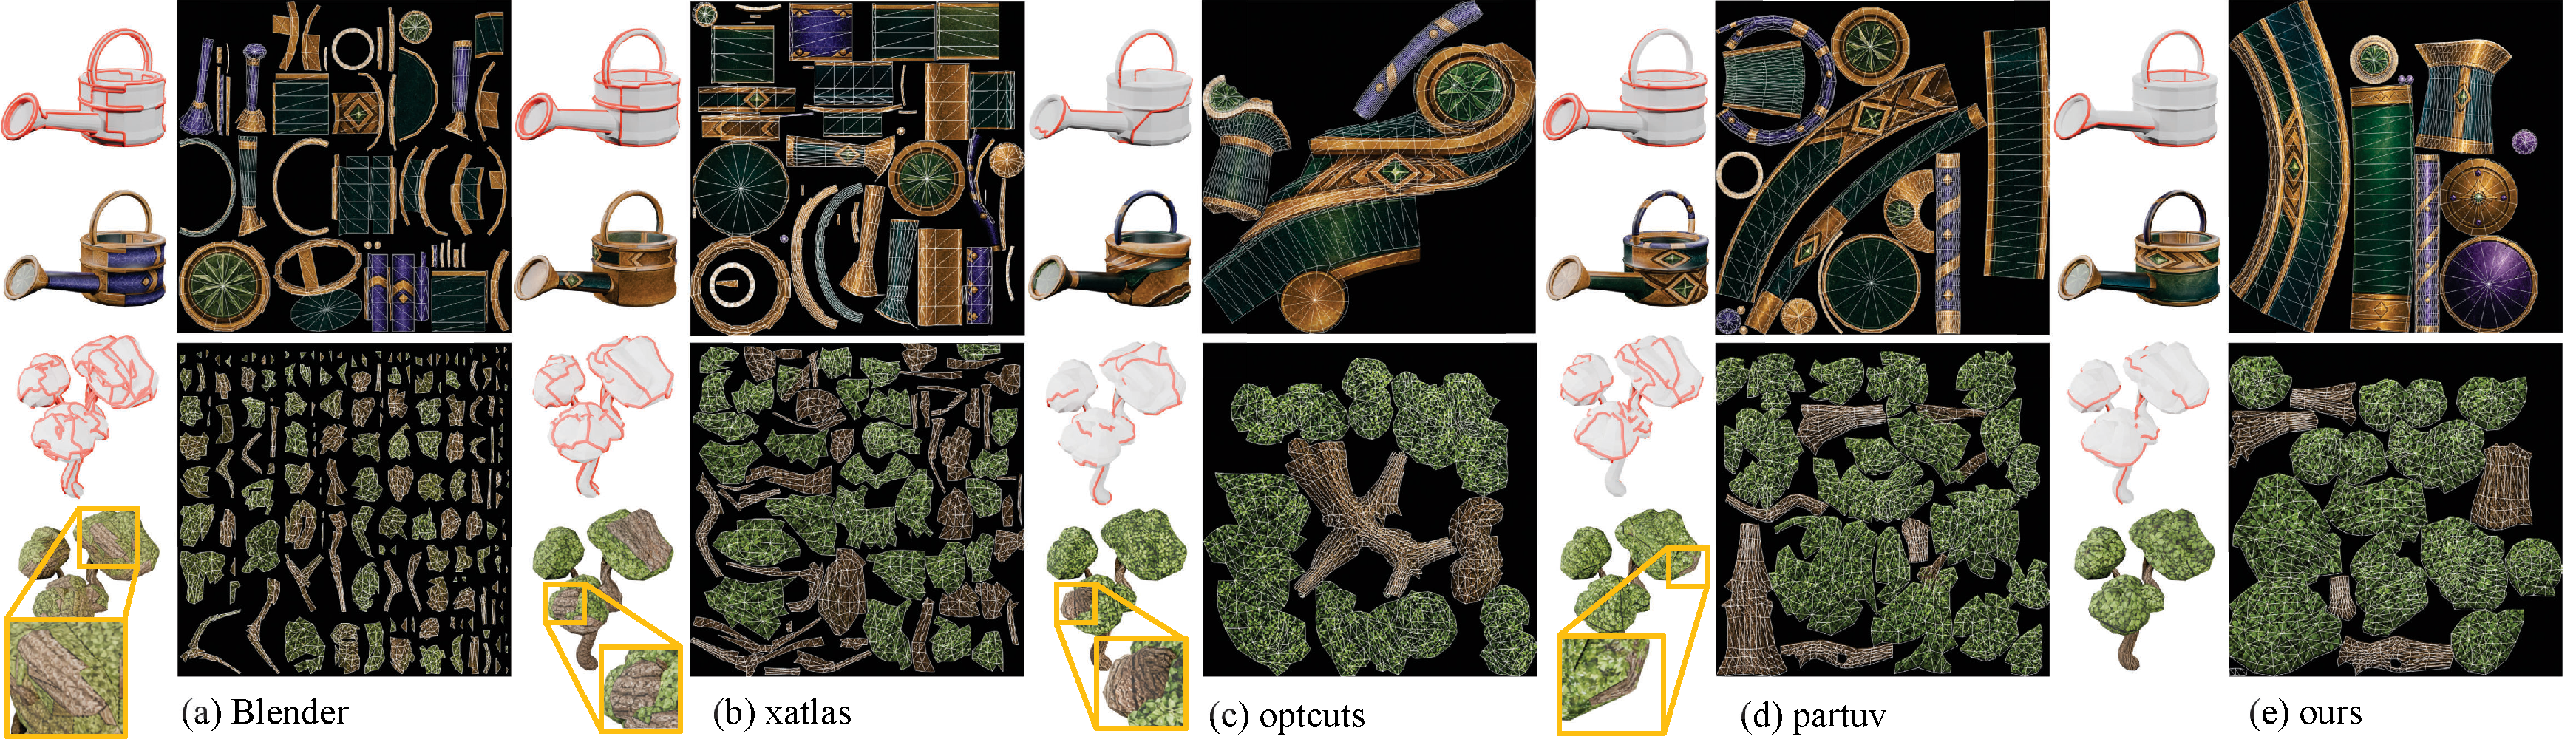
\includegraphics[width=\linewidth]{figures/comparison.pdf} 
    \caption{\textbf{Comparison.} We compare our \methodname{} against Blender's Smart UV Project~\cite{blender}, xatlas~\cite{young2019xatlas}, OptCuts~\cite{li2018optcuts}, and PartUV~\cite{wang2025partuv}.
    For each case, we show renderings with seams overlaid (upper left), the results of semantic-aware UV space texture generation (bottom left), and the corresponding UV space textures (right). Problematic regions are highlighted with yellow zoom-in boxes.
    } 
    \label{fig:comp_tex}
    \vspace{-4mm}
\end{figure*}

By alternating global context aggregation and local topology-aware update, the backbone captures both the global organization of seam layouts and the local evidence that determines where seams should lie. Since mesh edges are undirected, we process each edge in both directions during message passing and average the two directional edge features before prediction. The final edge features are normalized and projected to a scalar output for each mesh edge, yielding the edge-wise velocity field used in our flow matching model.

% Realizing the formulation above requires a neural architecture that parameterizes the velocity field directly on the mesh graph. Since the target seam layout is defined over mesh connectivity, a mesh-native graph network is a natural choice for this task. In particular, information propagation on the mesh graph provides an effective way to encode the local geometric structure that strongly influences seam placement.

% However, conventional graph neural networks (GNNs) are inherently local, with each layer propagating information only within a limited neighborhood, and capturing long range dependencies requires stacking many layers. This is problematic for seam generation: i) whether an edge should be selected as a seam often depends on its immediate geometric context, such as dihedral angle, local curvature, and proximity to sharp creases or part boundaries. ii) high quality seam layouts require global coordination across the entire surface, so that individual edge decisions collectively form connected, topologically valid cuts and partition the mesh into well shaped UV islands. Local information propagation alone is therefore insufficient to model the full seam layout distribution.

% To address this, we design a Mesh Transformer that combines local geometric aggregation with global context modeling (see the center of Fig.~\ref{fig:pipeline}). In each block, we first apply a global self-attention module over all vertices, allowing distant regions on the mesh to exchange information directly and enabling long-range coordination of seam decisions. We then apply a local message-passing module that updates vertex and edge features along mesh connectivity, refining predictions using local geometric structure in a topology-aware manner. By alternating these two modules throughout the network, our backbone captures both the local evidence and the global structural dependencies underlying artist-authored seam layouts, leading to seam predictions that are both geometrically precise and globally coherent.



\subsection{Conditional Seam Inpainting}
\label{sec:inpainting}
In production UV workflows, artists often refine an initial unwrap under partial constraints, such as protecting salient regions, enforcing selected seams, or revising charts that cause overlaps. 
We support this process with conditional seam inpainting, which reuses the learned flow model as a generative prior. 


Following conditional diffusion sampling~\cite{lugmayr2022repaint}, we clamp the known edges throughout the sampling process and let the model predict the unknown ones.
Let $\mathcal{K} \subset \mathcal{E}$ denote the set of known edges with target seam labels $e_1^{\mathcal{K}} \in \{0,1\}^{|\mathcal{K}|}$.
During sampling, we follow the same procedure as in unconditional generation, but overwrite the values of known edges at each step using their corresponding flow interpolation:
\[
e_{t,i} = t\, e_{1,i}^{\mathcal{K}} + (1-t)\, e_{0,i}, \quad i \in \mathcal{K},
\]
where $e_0$ is the initial Gaussian noise.
The updated $e_t$ is then passed to the Mesh Transformer for the next denoising step.
Because our backbone propagates information through both global self-attention and local message passing, the clamped edges serve as contextual constraints for the remaining editable edges, enabling coherent conditional seam generation.


This conditional inpainting mechanism enables two practical applications.
First, it supports constraint-guided seam completion.
Given sparse user-provided constraints, such as seam-free regions or edges that should be cut, \methodname{} resamples the unconstrained edges conditioned on these inputs.
The generated layout respects the prescribed constraints while remaining consistent with the learned artist-authored seam prior.
This provides a convenient form of coarse controllability: users specify high-level editing intent, and the model completes the remaining seam layout through conditional sampling.
Second, the same mechanism enables automatic localized self-refinement.
Since overlap-freeness is not explicitly enforced by the generative objective, a small number of sampled layouts may produce self-overlapping UV islands after parameterization.
For these cases, we keep the reliable parts of the seam layout fixed and treat only the region around the problematic island as editable.
Conditional inpainting then locally resamples seams in the affected region while preserving the rest of the layout.
This reuses the pretrained model as a local seam prior without requiring a separate repair network, additional training, or a handcrafted post-processing objective.

% In practical manual UV editing, artists interactively refine seams under partial constraints: certain visible or semantically important regions should remain seam-free, while some selected edges may be required as cuts to separate parts or resolve local parameterization issues. Since seam placement is inherently ambiguous and highly dependent on global shape context, completing the remaining layout from such partial constraints is difficult to achieve with handcrafted local rules. This motivates reusing the learned seam distribution as a conditional prior for interactive local seam editing.

% % Beyond unconditional seam generation, our trained flow model naturally supports training-free conditional seam inpainting. 
% Since seam layouts are represented as edge-wise variables on the mesh graph, any subset of edges can be treated as known conditions, while the remaining edges are regenerated by the same pretrained model. This allows \methodname{} to perform localized seam editing without training an additional model or optimizing a separate objective.

% Following the idea of conditional diffusion sampling~\cite{lugmayr2022repaint}, we clamp the known edges throughout the sampling process and let the model predict the unknown ones. Let $\mathcal{K} \subset \mathcal{E}$ denote the set of known edges with target seam labels $e_1^{\mathcal{K}} \in \{0,1\}^{|\mathcal{K}|}$. During sampling, we follow the same procedure as in unconditional generation, but overwrite the values of known edges at each step using their corresponding flow interpolation:
% \[
% e_{t,i} = t\, e_{1,i}^{\mathcal{K}} + (1-t)\, e_{0,i}, \quad i \in \mathcal{K},
% \]
% where $e_0$ is the initial Gaussian noise. The updated $e_t$ is then passed to the Mesh Transformer for the next denoising step. Since our backbone propagates information through both global self-attention and local message passing, the clamped edges provide contextual constraints for the remaining edges, enabling coherent local seam regeneration.

% This conditional inpainting mechanism enables two practical uses: constraint-guided seam generation and automatic self-refinement.
% First, it enables constraint guided local seam editing. Given user-provided sparse constraints, such as seam-free regions or edges to be cut, \methodname{} resamples the remaining unconstrained edges conditioned on these inputs, producing a seam layout that respects user intent while remaining consistent with the learned artist-authored distribution. This provides a convenient form of coarse local control, where users specify high-level constraints, and the model completes the layout through conditional sampling.
% %
% Second, the same mechanism can be used for automatic self-refinement. Since overlap-freeness is not explicitly enforced by the generative objective, a small number of sampled layouts may produce self-overlapping UV islands after parameterization. For these cases, we keep the reliable parts of the layout fixed and resample only a local region around the problematic island using conditional inpainting. This reuses the trained model as a local seam prior without requiring a separate repair model or additional training.
 

% Overall, post-sampling refinement does not require any extra training or separate optimization objective. It reuses the same generative model as a conditional seam prior, making \methodname{} applicable not only for fully automatic seam generation but also for interactive and localized UV layout correction.

% \subsection{Post-Sampling Refinement}
% \label{sec:refinement}
% After training, our model has learned to fit the distribution of artist-authored seam layouts, allowing it to generate seams that are globally plausible and consistent with artist-authored priors. However, since overlap-freeness is not explicitly enforced by the generative objective, distributional plausibility does not guarantee that every sampled seam layout can be flattened without error. This occasionally produces self-overlapping UV islands after parameterization.

% We address these failure cases through localized refinement. Rather than discarding the sample or introducing a separate repair model, we directly reuse the trained flow matching model for conditional seam inpainting. Specifically, \methodname{} admits standard training-free conditional sampling~\cite{lugmayr2022repaint} by fixing any subset of edges and using the pretrained model to generate the remaining edges without additional training. 
% Concretely, let $\mathcal{K} \subset \mathcal{E}$ denote the subset of edges with known target labels $e_1^{\mathcal{K}} \in {0,1}^{|\mathcal{K}|}$.
% During sampling, we follow the same procedure as in the base model, but for edges in $\mathcal{K}$, we replace their current values with the linear interpolation between the target seam labels and the initial noise,
% \[
% e_{t,i} = t\, e_{1,i}^{\mathcal{K}} + (1-t)\, e_{0,i}, \quad i \in \mathcal{K},
% \]
% and then feed the updated $e_t$ into the model for the next step. Since the Mesh Transformer propagates information through both global self-attention and local message passing, the clamped known edges condition the velocity predictions for the remaining edges throughout the denoising process.

 
% Based on the conditional inpainting mechanism which naturally supports localized UV correction and inspired by practical manual UV editing, 
% % when artists encounter an overlapping island, they may either insert additional seams inside the island to further subdivide it, or locally adjust the partition between the island and its neighboring regions. 
% we consider two refinement modes as shown in the Fig~\ref{fig:refine}. 

% % The first keeps the island boundary fixed and only re-generates seams in the interior, corresponding to local subdivision within the problematic island. 

% The first mode keeps the island boundary fixed and only re-generates seams in the interior, corresponding to local subdivision within the problematic island. Let $I$ be an overlapping island and let $\mathcal{E}^{\mathrm{int}}(I) \subset \mathcal{E}$ denote the edges strictly interior to $I$, i.e., edges whose endpoints both lie away from the UV boundary of $I$. We define the known subset as
% \[
% \mathcal{K}_{\mathrm{int}} = \mathcal{E} \setminus \mathcal{E}^{\mathrm{int}}(I),
% \]
% clamp $\mathcal{K}_{\mathrm{int}}$ to the current seam labels, and re-inpaint only $\mathcal{E}^{\mathrm{int}}(I)$. Because the boundary of $I$ is preserved, the rest of the atlas remains unchanged, and any newly introduced cuts can only appear inside $I$, subdividing it into smaller sub-islands. This mode is effective when the overlap is caused by insufficient internal seams.

% When modifying the island interior alone is not sufficient, we switch to the second mode.
% % and enlarge the resampled region around the problematic island. 
% The second allows a larger local neighborhood around the island boundary to be re-generated, so that the island can be repartitioned together with its immediate neighbors while the rest of the atlas remains fixed.
% Let $\mathcal{N}(I)$ denote the set of UV islands that share at least one boundary edge with $I$, and let $\mathcal{E}^{\mathrm{bd}}(I)$ denote the boundary edges of $I$. We define the resampled region as
% \[
% \mathcal{U}_{\mathrm{bd}} = \mathcal{E}^{\mathrm{bd}}(I) \;\cup\; \bigcup_{J \in \mathcal{N}(I)} \mathcal{E}^{\mathrm{int}}(J),
% \]
% and use
% \[
% \mathcal{K}_{\mathrm{bd}} = \mathcal{E} \setminus \mathcal{U}_{\mathrm{bd}}
% \]
% as the known subset. Clamping $\mathcal{K}_{\mathrm{bd}}$ and re-inpainting $\mathcal{U}_{\mathrm{bd}}$ allows the problematic island to grow or shrink against its immediate neighbors, while keeping regions beyond the 1-hop neighborhood fixed. This provides greater flexibility when the overlap is rooted in an unsuitable local boundary partition rather than a lack of internal seams.

% \begin{figure}[t]
%     \centering
%     \includegraphics[width=\linewidth]{figures/inpainting.pdf}
%     \caption{\textbf{Two modes of \methodname{} refinement.}}
%     \label{fig:refine}
% \end{figure}



\begin{table*}[t]
\definecolor{valColor}{RGB}{255, 245, 235}  % 淡橙 (Seam Graph)
    \definecolor{wildColor}{RGB}{235, 245, 255} % 淡蓝 (UV Islands)
    \definecolor{distColor}{RGB}{240, 252, 239} % 淡绿 (Distortion & Time)
    \definecolor{userColor}{RGB}{248, 240, 252} % 淡紫 (User Pref)
     \definecolor{1st}{HTML}{F8CBA6}
    \definecolor{2nd}{HTML}{FFE7CC}
    \centering
    \caption{\textbf{Quantitative comparisons.}
We evaluate seam generation performance using layout, distortion, runtime, and perceptual metrics. 
For layout statistics, we directly report the number of seam edges and UV islands, where values closer to the ground truth are better. 
We also report standard distortion metrics, runtime, and preference scores from both large vision-language models and human users.
\methodname{} achieves the closest layout statistics to the ground truth while obtaining the highest perceptual preference scores with comparable distortion and runtime.
\textcolor{1st}{$\blacksquare$} and \textcolor{2nd}{$\blacksquare$} and denote the 1st and 2nd places.
% The best result is highlighted in bold, and the second best is underlined.
% , including {the number of seam edges and UV island fragmentation}, {distortion}, {runtime}, and preference scores from both real users and large vision language models.
% \methodname{} consistently matches the ground-truth statistics more closely than baselines while maintaining superior efficiency and visual quality.
% The 1st place is denoted in bold, and the 2nd place is underlined. 
% ``$\sim 1$'' indicates that values closer to 1 are better.
}
    \label{tab:structure}
    % \vspace{2pt}
    \small
    \setlength{\tabcolsep}{4.5pt} % 略微缩小间距以适应更多列
    \renewcommand{\arraystretch}{1.3}
    \resizebox{0.85\linewidth}{!}{
    % \begin{tabular}{l cccccc ccc cc}
    \begin{tabular}{l cc ccc cc}
        \toprule
        Method
        & \textbf{VLM Score} $\uparrow$
        & \textbf{User Pref.} $\uparrow$ 
        & \textbf{\#Seam Edges $\sim GT$} 
        & \textbf{\#Islands $\sim GT$} 
        & \textbf{Ang. Distort.} $\sim 1$ 
        & \textbf{Area Distort.} $\sim 1$ 
        & \textbf{Running Time (s)} $\downarrow$ 
        \\
        \midrule
        
        Ground Truth 
        & -- 
        & -- 
        & 476.6  
        & 67.8  
        & 0.9110 
        & 2.4238  
        & -- 
        
        \\
        \midrule

        Blender 
        & 2.33  
        & 2.37 
        & 800.7  
        & 133.6 
        & 0.9207 
        & 1.1120 
        & \cellcolor{1st}{0.008} 
        
        \\
        
        xatlas 
        & 2.71 
        & 2.34 
        & 722.8  
        & 110.8  
        & \cellcolor{1st}{0.9817} 
        & \cellcolor{2nd}{1.0852} 
        & \cellcolor{2nd}{0.137}  
       
        \\
        
        optcuts 
        & 2.93  
        & 2.58 
        & 144.4  
        & 4.6  
        & 0.8845 
        & 1.1718 
        & 568.53  
        \\
        
        PartUV 
        & \cellcolor{2nd}{3.02} 
        & \cellcolor{2nd}{2.91}  
        & \cellcolor{2nd} 628.1  
        & \cellcolor{2nd} 96.1 
        & \cellcolor{2nd}{0.9749} 
        & \cellcolor{1st}{1.0843} 
        & 1.17 

        \\
        
        \methodname{} (Ours) 
        & \cellcolor{1st}{3.56} 
        & {\cellcolor{1st}{4.37}} 
        & {\cellcolor{1st} 471.5}  
        & {\cellcolor{1st}62.7}  
        & 0.9421 
        & 1.9087 
        & 2.87  
        \\
        
        \bottomrule
    \end{tabular}
    }
\end{table*}


\section{Experiments}
In this section, we first introduce the implementation details of \methodname{} (Sec.~\ref{sec:impl}), then present comparisons with state of the art methods (Sec.~\ref{sec:Comparison}), evaluate the effectiveness of each component through ablation studies (Sec.~\ref{sec:ablation}).We then demonstrate additional qualitative results, including symmetric seam layouts and component-wise UV generation for complex assets (Sec.~\ref{sec:additional_results}) and finally demonstrate inpainting applications (Sec.~\ref{sec:app_inpainting}).


\subsection{Implementation Details}
\label{sec:impl}
We collect artist-authored UV layouts from publicly available 3D assets, including meshes from Objaverse~\cite{objaverse,objaverseXL} and Sketchfab. 
% We retain models with valid UV parameterizations and extract seam labels from their UV island boundaries. 
We train the flow matching stage for 200 epochs on 8 NVIDIA A100 GPUs, using the AdamW optimizer with a fixed learning rate of $1\times10^{-5}$ and a batch size of 16.  
We use the $x$-prediction parameterization together with the $v$ loss for training. During training, each mesh is augmented with random rotations to improve generalization. At inference time, the final continuous seam predictions are binarized using a threshold of $\tau = 0.0$. We then use Blender's Python API to unwrap each mesh with the extracted seams using the angle-based unwrapping method. Detailed network architecture parameters, dataset collection and preprocessing procedures are provided in the supplementary material.



\subsection{Comparison}
\label{sec:Comparison}
% We evaluate our \methodname{} on a held-out validation set of 200 meshes against four state-of-the-art automatic UV unwrapping methods: Blender's Smart UV Project~\cite{blender}, xatlas~\cite{young2019xatlas}, OptCuts~\cite{li2018optcuts}, and PartUV~\cite{wang2025partuv}.
We compare \methodname{} with automatic UV unwrapping baselines: Blender's Smart UV Project~\cite{blender}, xatlas~\cite{young2019xatlas}, OptCuts~\cite{li2018optcuts}, and PartUV~\cite{wang2025partuv}.

\subsubsection{Qualitative Comparison}
\label{sec:qualitative}

We show qualitative comparisons in Fig.~\ref{fig:qualitative}. 
Blender~\cite{blender} and xatlas~\cite{young2019xatlas} often over-fragment the surface into many small UV islands, resulting in dense seam cuts that can break semantic coherence and pass through visually prominent regions. 
OptCuts~\cite{li2018optcuts} produces more consolidated charts, often mapping each connected surface region to a single large island, but the resulting island boundaries tend to be distorted and less aligned with semantic parts. 
PartUV~\cite{wang2025partuv} mitigates over-fragmentation by incorporating semantic part priors. 
However, its distortion-driven flattening process may still disrupt semantic continuity, resulting in seams that occasionally appear in visually important regions.
% Blender's Smart UV Project~\cite{blender} tends to over-segment the surface into many small, irregularly shaped charts. Xatlas~\cite{young2019xatlas} generates more conservative cuts but often places seams through visually prominent regions such as the front face or the chest of a character, which may lead to noticeable texture discontinuities after texturing. 
% PartUV, although guided by semantic part segmentation, often introduces excessive seams and produces overly fragmented chart decompositions, with some seams placed in visually important regions.
%
In contrast, \methodname{} produces more coherent seam layouts with fewer fragmented cuts and better-shaped UV islands. 
The generated seams are often aligned with natural geometric boundaries, such as creases, part junctions, and occluded regions, while avoiding visually prominent areas. 
This leads to more artist-friendly UV decompositions for downstream texture editing.

We further assess the semantic quality of UV layouts through their compatibility with 2D generative priors. Specifically, we use GPT-Image-2~\cite{openai2026gptimage2} to synthesize textures directly in UV space from position and normal maps (Fig.~\ref{fig:comp_tex}). Since 2D trained models naturally generate continuous textures within connected regions, the synthesis quality serves as a proxy for the semantic coherence and continuity of the UV layout.
%
Baselines with highly fragmented UV charts often destroy global semantic context, leading to severe color bleeding and disjointed patterns due to insufficient structural continuity across isolated islands.
%
In contrast, our approach preserves contiguous semantic regions, significantly mitigating these artifacts and producing highly coherent textures.
% This directly benefits downstream workflows, as texture artists can paint across larger and more contiguous UV regions with less need to handle fragmented charts. 
% Furthermore, \methodname{} places seams along natural geometric boundaries such as sharp creases, part junctions, and occluded regions (e.g., the inner side of limbs or the underside of a model), where seams are less perceptible, reduce visible texture discontinuities, and better preserve continuity in visually salient regions. 
% It is also notably restrained in visually important regions such as the face, reflecting the common artist preference to keep these areas as intact as possible. 
% Overall, these results suggest that \methodname{} produces seam layouts that are better aligned with practical artist workflows.

% \textbf{Semantic-Aware UV-space Texture Generation.} 
% We further assess the semantic quality of our UV maps by examining their compatibility with 2D generative priors. Specifically, we utilize GPT-Image-2.0~\cite{openai2026gptimage2} to synthesize textures directly in the UV space, conditioned on position and normal maps (Fig.~\ref{fig:comp_tex}). 
% %
% Since models trained in 2D naturally synthesize continuous texture within connected regions, the quality of the synthesized output serves as a proxy for the UV layout's capability to yield semantically-cohesive and contiguous islands.
%
% Baselines that produce highly fragmented UV charts inherently destroy the global semantic context. Specifically, this over-segmentation frequently leads to severe color bleeding and disjointed patterns, as the isolated islands fail to provide sufficient structural cues. 


% \begin{figure}[t]
%     \centering
%     \includegraphics[width=\linewidth]{figures/diversity.pdf}
%     \caption{\textbf{Diverse seam layouts} generated by \methodname{} for the same input mesh. Different samples of the initial noise $e_0 \sim \mathcal{N}(0, I)$ are denoised through the same learned flow, producing multiple plausible seam placements that each represent a valid artistic choice.}
%     \label{fig:diversity}
% \end{figure}

% \paragraph{Generation Diversity.}
% As a generative model, \methodname{} is capable of producing multiple distinct yet plausible seam layouts for the same input mesh. Since the flow matching formulation starts from a randomly sampled initial noise $e_0 \sim \mathcal{N}(0, I)$, different noise samples are transported through the learned flow to arrive at different clean predictions, naturally yielding diverse seam placements as shown in Fig.~\ref{fig:diversity}. Each generated layout respects geometric boundaries and maintains topological validity, yet exhibits meaningfully different cut paths. This diversity reflects the inherent ambiguity in UV unwrapping—there is no single correct answer, and different artists may prefer different cuts depending on the intended texture style or painting workflow. The ability to offer multiple candidate layouts from different initial noise samples provides practical flexibility: users can select the most suitable unwrapping for their specific downstream task, a capability that deterministic methods fundamentally cannot provide.





% \begin{table*}[t]
%     \centering
%     \caption{\textbf{Ablation on backbone design and inference procedure.} \emph{w/o inpainting} disables the progressive overlap resolution at inference and reports the single-shot generation result; \emph{w/o Global Attn.} removes the global self-attention stream; \emph{Naive GraphConv} replaces the local attention module with a vanilla graph convolution while keeping the global stream. Lower predicted overlap rate is better.}
%     \label{tab:ablation}
%     \vspace{2pt}
%     \resizebox{0.6\linewidth}{!}{%
%     \begin{tabular}{l c c c c}
%         \toprule
%         Metric & \methodname{} (Full) & w/o inpainting & w/o Global Attn. & Naive GraphConv \\
%         \midrule
%         Pred Overlap Rate $\downarrow$ & \textbf{3.5\%} & 26.5\% & 48.1\% & 72.6\% \\
%         \bottomrule
%     \end{tabular}%
%     }
% \end{table*}
% \begin{table}[t]
%     \centering
%     \caption{\textbf{Ablation on backbone design and inference procedure.}
%     We report the predicted overlap rate after UV parameterization; lower is better.
%     \emph{w/o self-refinement} disables automatic overlap correction and directly evaluates the initially sampled seam layout.
%     \emph{w/o Global Attn.} removes the global self-attention stream.
%     \emph{Naive GraphConv} replaces the local attention module with a vanilla graph convolution while keeping the global stream.}
%     \label{tab:ablation}
%     \vspace{2pt}
%     \begin{tabular}{l c}
%         \toprule
%         Variant & Pred. Overlap Rate $\downarrow$ \\
%         \midrule
%         \methodname{} & 26.5\% \\
%         \methodname{} (self-refined) & \textbf{3.5\%} \\
%         w/o Global Attn. & 48.1\% \\
%         Naive GraphConv & 72.6\% \\
%         \bottomrule
%     \end{tabular}
% \end{table}



\subsubsection{Quantitative Comparison}
\label{sec:quantitative}
We use a held-out validation set of 200 meshes for evaluation. 
OptCuts only successfully processes 170 out of the 200 validation meshes due to its stricter input requirements; we therefore report its statistics on these valid cases. All other methods are evaluated on the full validation set.

\begin{figure}[t]
    \centering
    
\includegraphics[width=\linewidth]{figures/ablation.pdf}
    \caption{\textbf{Backbone design ablation.}
    Compared to the full model, removing global self-attention leads to less coordinated seam layouts and irregular UV partitions, while replacing local attention with a naive graph convolution produces less geometry-aware cuts and poorly organized UV islands.}
    \vspace{-6mm}
    \label{fig:ablation}
\end{figure}

As shown in Tab.~\ref{tab:structure}, we first evaluate the perceptual quality of the generated seam layouts using both automated and human assessments.
For the VLM-based evaluation, we concatenate anonymized UV layouts from all methods into a randomized panel for each test example and ask Gemini-2.5-Flash~\cite{gemini25} to assign a 1--5 quality score to each layout.
\methodname{} achieves the highest average VLM score, suggesting better structural clarity and paintability under this standardized evaluation protocol.
We further conduct a user study to assess human preference.
Twenty participants with 3D texturing experience rate each result on a 1--5 scale based on seam naturalness, chart coherence, and suitability for texture editing.
\methodname{} receives the highest average score, further confirming its alignment with artist-oriented UV editing criteria.
We then compare basic layout statistics, including the number of seam edges and the number of UV islands.
These measures reflect whether a method produces cuts and chart decompositions at a granularity similar to artist-authored layouts.
\methodname{} is closest to the ground truth on both measures, indicating that the learned generative prior captures the overall cutting style of professional UV layouts.
Finally, we report traditional geometric metrics, including distortion and runtime.
Interestingly, the ground-truth artist-authored layouts have the worst area distortion and the second-worst angular distortion among all methods, suggesting that distortion minimization is not the primary goal of professional seam placement.
Although \methodname{} does not explicitly optimize distortion objectives, it achieves angular distortion comparable to existing automatic unwrapping methods, while its area distortion remains within a reasonable range.
In terms of runtime, \methodname{} is slightly slower than Blender, xatlas, and PartUV, but much faster than OptCuts, providing a practical trade-off between artist-aligned seam quality and efficiency.

Further details, including  additional seam and island structure statistics, metric definitions, user-study examples, VLM prompts, and representative VLM evaluations, are provided in the supplementary material.
% As shown in Tab.~\ref{tab:structure}, we first compare basic layout statistics, including the number of seam edges and the number of UV islands. 
% These measures reflect whether a method produces cuts and chart decompositions at a granularity similar to artist-authored layouts. 
% \methodname{} is closest to the ground truth on both measures, indicating that the learned generative prior captures the overall cutting style of professional UV layouts. 
% Additional seam and island structure statistics are provided in the supplementary material.
% We also evaluate traditional geometric metrics, including distortion and runtime. 
% Interestingly, the ground-truth artist-authored layouts have the worst area distortion and the second-worst angular distortion among all methods, suggesting that distortion minimization is not the primary goal of professional seam placement. 
% Although \methodname{} does not explicitly optimize distortion objectives, it achieves angular distortion comparable to existing automatic unwrapping methods, while its area distortion remains within a reasonable range. 
% In terms of runtime, \methodname{} is slightly slower than Blender, xatlas, and PartUV, but much faster than OptCuts, providing a practical trade-off between artist-aligned seam quality and efficiency.
% To provide an automated perceptual proxy, we further conduct a VLM-based evaluation. 
% For each test example, we concatenate anonymized UV layouts from all methods into a randomized panel and ask Gemini-2.5-Flash~\cite{gemini25} to assign a 1--5 quality score to each layout. 
% \methodname{} achieves the highest average VLM score, suggesting better structural clarity and paintability under this standardized evaluation protocol.
% Finally, we conduct a user study to assess human preference. 
% Twenty participants with 3D texturing experience rate each result on a 1--5 scale based on seam naturalness, chart coherence, and suitability for texture editing. 
% \methodname{} receives the highest average score, further confirming its alignment with artist-oriented UV editing criteria.
% Further details, including metric definitions, user-study examples, VLM prompts, representative VLM evaluations, are provided in the supplementary material.
% We further evaluate all methods using traditional measures of distortion and runtime performance.

% Although existing methods explicitly optimize distortion based objectives, \methodname{} does not incorporate such terms, yet still achieves angular distortion comparable to state of the art methods. While its area distortion is slightly higher than that of the best performing baselines, it remains better than the ground truth. This suggests that the learned prior implicitly captures distortion related properties despite the absence of explicit supervision.
% Runtime ranges from 0.008 s to 568.53 s across methods, while \methodname{} runs at 2.87 s, offering a favorable trade-off between efficiency and quality.

% As demonstrated in Tab.~\ref{tab:structure}, although the validation set consists of unseen cases, \methodname{} significantly outperforms existing baselines in replicating professional seam cut logic, thanks to the learned generative distribution.
 
% While prior heuristic-based or optimization-driven frameworks often achieve superior performance on traditional geometric metrics like distortion, they frequently fail to capture the high-level seam placement logic of professional workflows. 
% Therefore, we conduct a user study to evaluate perceptual quality. 20 participants assigned scores on a scale of 1 to 5 based on the naturalness and visibility of seam placement, the coherence of chart boundaries, and the suitability of the resulting UV islands for practical texture editing. Further details regarding metric definitions, user study examples and additional quantitative analyses are provided in the supplementary material. \methodname{} achieves the highest human preference score.

% We further conduct a VLM-based evaluation to assess the structural quality and paintability of UV layouts.
% For each test example, we concatenate the UV layouts produced by five methods into a single panel, randomize their order, and ask Gemini-2.5-Flash~\cite{gemini25} to assign a 1--5 quality score to each anonymized layout.
% We compute the final VLM score of each method by averaging its assigned quality scores over all evaluated examples.
% \methodname{} receives the highest average VLM score among all evaluated methods, suggesting that its UV layouts better align with artist-oriented perceptual criteria captured by the vision-language model. 

% In the supplementary material, we further provide additional evaluation results, including the full VLM prompts, representative evaluation examples, and additional comparisons of seam statistics.

% Further details, including the full VLM prompt and representative evaluation examples, are provided in the supplementary material.

% Since \methodname{} models artist-authored seam distributions rather than optimizing a fixed handcrafted objective, we evaluate each method by comparing structural statistics against the ground truth at both the seam-graph and UV-island levels.
% The main paper reports six representative metrics in Tab.~\ref{tab:structure}: the number of seam edges, path edge ratio, and junction ratio for seam-graph structure, and the number of islands, largest island ratio, and tiny-island count ratio for UV-island decomposition.
% These metrics measure the amount of cutting, seam connectivity, branching complexity, atlas fragmentation, and the preservation of large contiguous charts.
% Values closer to the ground truth indicate better agreement with the structural organization of artist-authored seam layouts.
% Additional metrics are provided in the supplementary material.

% As shown in Tab.~\ref{tab:structure}, \methodname{} achieves the closest match to the ground truth across the representative seam-graph and UV-island metrics.
% At the seam-graph level, our method closely matches the overall number of seam edges, avoids excessive branching, and produces coherent path-like seam structures.
% In contrast, Blender, xatlas, and PartUV tend to introduce more cuts, while OptCuts produces an overly coarse decomposition.
% At the island level, \methodname{} generates a number of UV islands close to the ground truth, preserves larger contiguous regions, and avoids excessive tiny charts.
% Overall, these results show that \methodname{} better captures the structural distribution of artist-authored seam layouts than competing methods.








% We evaluate \methodname{} on a held-out validation set of 200 meshes, with the goal of verifying whether the generated seam layouts better match the distribution of artist-authored seams. 
% To this end, we compare \methodname{} against four representative automatic UV unwrapping methods: Blender's Smart UV Project~\cite{blender}, a projection-based tool that segments meshes by face normal clustering; xatlas~\cite{young2019xatlas}, a chart-growing algorithm that iteratively merges regions under distortion bounds; OptCuts~\cite{li2018optcuts}, an optimization-based method that jointly determines surface cuts and parameterization to reduce distortion; and PartUV~\cite{wang2025partuv}, a learning-based method that combines semantic part segmentation with geometric flattening heuristics. 
% Due to its stricter input requirements, OptCuts successfully processes 129 out of the 200 validation meshes; we therefore report its statistics on these successfully processed cases, while all other methods are evaluated on the full validation set.
% Since our method is trained to model the distribution of human-authored seam layouts rather than optimize a fixed handcrafted objective, we evaluate all methods by comparing the structural statistics of their generated seams against the ground truth at both the seam-graph level and the UV-island level.
% We evaluate \methodname{} on a held-out validation set of 200 meshes, with the goal of verifying whether the generated seam layouts better match the distribution of artist-authored seams. To this end, we compare \methodname{} against three automatic UV unwrapping methods: Blender's Smart UV Project~\cite{blender}, a projection-based tool that segments meshes by face normal clustering; xatlas~\cite{young2019xatlas}, a chart-growing algorithm that iteratively merges regions under distortion bounds; and PartUV~\cite{wang2025partuv}, a learning-based method that combines semantic part segmentation with geometric flattening heuristics. Since our method is trained to model the distribution of human-authored seam layouts rather than optimize a fixed handcrafted objective, we evaluate all methods by comparing the structural statistics of their generated seams against the ground truth at both the seam-structure level and the UV-island level.

% \paragraph{Evaluation metrics.}
% We evaluate predicted seam layouts using structural statistics of both the seam graph and the resulting UV-island decomposition. 
% While we provide a more complete set of metrics in the supplementary material, the main paper reports six representative metrics in Tab. ~\ref{tab:structure} for a focused comparison. 
% For the seam graph, we use the \textbf{number of seam edges}, \textbf{path edge ratio}, and \textbf{junction ratio}, which respectively measure the overall amount of cutting, the extent to which seam edges form coherent path-like components, and the frequency of branching points with vertex degree $\geq 3$. 
% These metrics capture whether the generated seams form clean and usable chart boundaries rather than overly fragmented or highly branched structures.
% For the \emph{UV islands}, we use the \textbf{number of islands}, \textbf{largest island ratio}, and \textbf{tiny island count ratio}, which characterize the degree of chart decomposition, the preservation of large contiguous editable regions, and the amount of small fragmented charts. 
% These metrics are closely related to practical downstream use, since layouts with excessive islands or many tiny charts are cumbersome for texture painting and packing, while artist-authored UVs typically concentrate surface area into a moderate number of meaningful charts. 
% For all metrics, values closer to the ground-truth statistics indicate that the predicted seam layout better matches the structural organization of artist-authored reference seams. The supplementary material provides a more complete evaluation with additional statistics, including loop-edge ratio, seam-component coverage, tiny-island area ratio, and $N90$.



% \begin{table*}[t]
%     \centering
%     \caption{\textbf{Comparison of seam-structure statistics on the held-out validation set.} We report the number of seam edges, path edge ratio, loop edge ratio, junction ratio, and top-3 coverage, which together characterize the amount of cutting, the connectivity pattern, and the structural concentration of the seam graph. Since our goal is to match the distribution of artist-authored seam layouts, values closer to the ground-truth statistics are preferred. Best results are shown in \textbf{bold}.}
%     \label{tab:seam}
%     \vspace{2pt}
%     \begin{tabular}{l c c c c c}
%         \toprule
%         Method & \#Edges & Path Edge Ratio & Loop Edge Ratio & Junc. Ratio & Top-3 Cov. \\
%         \midrule
%         Blender~\cite{blender}        & 800.7 & 0.41  & 0.95 & 17.75 & 65.53 \\
%         xatlas~\cite{young2019xatlas} & 722.8 & 1.40  & 2.43 & 16.97 & 67.07 \\
%         optcuts~\cite{li2018optcuts}  & 144.4 & 38.6   & 0.0 & 3.62 & 85.5 \\
%         PartUV~\cite{wang2025partuv}  & 628.1 & 4.35  & 3.18 & 13.24 & 72.63 \\
%         \midrule
%         \methodname{} (Ours)          & \textbf{471.5} & \textbf{13.15} & \textbf{9.23} & \textbf{9.02} & \textbf{68.15} \\
%         Ground Truth                  & 476.6 & 11.35 & 8.91 & 8.96 & 69.39 \\
%         \bottomrule
%     \end{tabular}
% \end{table*}

% \begin{table*}[t]
%     \centering
%     \caption{\textbf{Comparison of UV-island statistics on the held-out validation set.} We report the number of islands, largest island ratio, top-3 coverage, tiny island count ratio, tiny island area ratio, and $N90$, which together characterize the number of UV charts and their area distribution. Since our goal is to match the distribution of artist-authored seam layouts, values closer to the ground-truth statistics are preferred. Best results are shown in \textbf{bold}.}
%     \label{tab:island}
%     \vspace{2pt}
%     \begin{tabular}{l c c c c c c}
%         \toprule
%         Method & \#Islands & Largest Ratio & Top-3 Cov. & Tiny Count Ratio & Tiny Area Ratio & $N90$ \\
%         \midrule
%         Blender~\cite{blender}        & 133.6 & 15.54 & 37.65 & 60.71 & 9.88 & 41.1 \\
%         xatlas~\cite{young2019xatlas} & 110.8 & 17.10 & 39.34 & 54.46 & 7.93 & 34.1 \\
%         optcuts~\cite{li2018optcuts}  & 4.57 & 72.5 & 91.5 & 7.33 & 0.17 & 2.81 \\
%         PartUV~\cite{wang2025partuv}  & 96.1 & 27.27 & 53.71 & 39.61 & 6.28 & 31.8 \\
%         \midrule
%         \methodname{} (Ours)          & \textbf{62.7} & \textbf{37.85} & \textbf{63.28} & \textbf{35.88} & \textbf{5.03} & \textbf{22.64} \\
%         Ground Truth                  & 67.8 & 35.10 & 60.16 & 33.48 & 4.91 & 	24.19 \\
%         \bottomrule
%     \end{tabular}
% \end{table*}

% \begin{table*}[t]
%     \centering
%     \caption{\textbf{Comparison of seam-graph and UV-island structure statistics on the held-out validation set.}
% We compare automatic methods against artist-authored ground truth using representative statistics that describe the amount of cutting, seam-graph connectivity, and UV-atlas fragmentation.
% Since our goal is to reproduce the distribution of artist-authored seam layouts, values closer to the ground-truth statistics are preferred, and the closest method result is shown in \textbf{bold}.
% \methodname{} consistently matches the ground truth most closely across all reported metrics, producing a comparable number of seam edges, similar path and junction ratios, and UV islands with fragmentation statistics closest to artist-authored layouts.
% In contrast, heuristic methods tend to over-fragment the atlas, while OptCuts produces overly coarse decompositions with too few seams and islands.}
%     \label{tab:structure}
%     \vspace{2pt}
%     \begin{tabular}{l c c c c c c}
%         \toprule
%         Method 
%         & \multicolumn{3}{c}{Seam Graph}
%         & \multicolumn{3}{c}{UV Islands} \\
%         \cmidrule(lr){2-4} \cmidrule(lr){5-7}
%         & \#Seam Edges 
%         & Path Ratio 
%         & Junc. Ratio 
%         & \#Islands 
%         & Largest Ratio 
%         & Tiny Count Ratio \\
%         \midrule
%         Blender~\cite{blender}        
%         & 800.7 & 0.41  & 17.75 & 133.6 & 15.54 & 60.71 \\
%         xatlas~\cite{young2019xatlas} 
%         & 722.8 & 1.40  & 16.97 & 110.8 & 17.10 & 54.46 \\
%         optcuts~\cite{li2018optcuts}  
%         & 144.4 & 38.60 & 3.62  & 4.57  & 72.50 & 7.33 \\
%         PartUV~\cite{wang2025partuv}  
%         & 628.1 & 4.35  & 13.24 & 96.1  & 27.27 & 39.61 \\
%         \midrule
%         \methodname{} (Ours)          
%         & \textbf{471.5} 
%         & \textbf{13.15} 
%         & \textbf{9.02} 
%         & \textbf{62.7} 
%         & \textbf{37.85} 
%         & \textbf{35.88} \\
%         Ground Truth                  
%         & 476.6 & 11.35 & 8.96 & 67.8 & 35.10 & 33.48 \\
%         \bottomrule
%     \end{tabular}
% \end{table*}

% \begin{table*}[t]
%     \centering
%     \caption{\textbf{Comparison of seam-graph and UV-island structure statistics on the held-out validation set.}
%     We compare automatic methods against artist-authored ground truth using representative statistics that describe the amount of cutting, seam-graph connectivity, and UV-atlas fragmentation.
%     Since our goal is to reproduce the distribution of artist-authored seam layouts, values closer to the ground-truth statistics are preferred.
%     We additionally report the absolute difference to ground truth, denoted by $\lvert \Delta_{\mathrm{GT}} \rvert = \lvert x - x_{\mathrm{GT}} \rvert$, where lower is better.
%     The closest method result and the smallest $\lvert \Delta_{\mathrm{GT}} \rvert$ are shown in \textbf{bold}.
%     \methodname{} consistently matches the ground truth most closely across all reported metrics, producing a comparable number of seam edges, similar path and junction ratios, and UV islands with fragmentation statistics closest to artist-authored layouts.
%     In contrast, heuristic methods tend to over-fragment the atlas, while OptCuts produces overly coarse decompositions with too few seams and islands.}
%     \label{tab:structure}
%     \vspace{2pt}

%     \small
%     \setlength{\tabcolsep}{3.5pt}
%     \begin{tabular}{l cc cc cc cc cc cc}
%         \toprule
%         Method 
%         & \multicolumn{6}{c}{Seam Graph}
%         & \multicolumn{6}{c}{UV Islands} \\
%         \cmidrule(lr){2-7} \cmidrule(lr){8-13}
%         & \multicolumn{2}{c}{\#Seam Edges}
%         & \multicolumn{2}{c}{Path Ratio}
%         & \multicolumn{2}{c}{Junc. Ratio}
%         & \multicolumn{2}{c}{\#Islands}
%         & \multicolumn{2}{c}{Largest Ratio}
%         & \multicolumn{2}{c}{Tiny Count Ratio} \\
%         \cmidrule(lr){2-3}
%         \cmidrule(lr){4-5}
%         \cmidrule(lr){6-7}
%         \cmidrule(lr){8-9}
%         \cmidrule(lr){10-11}
%         \cmidrule(lr){12-13}
%         & Value & $\lvert \Delta_{\mathrm{GT}} \rvert \downarrow$
%         & Value & $\lvert \Delta_{\mathrm{GT}} \rvert \downarrow$
%         & Value & $\lvert \Delta_{\mathrm{GT}} \rvert \downarrow$
%         & Value & $\lvert \Delta_{\mathrm{GT}} \rvert \downarrow$
%         & Value & $\lvert \Delta_{\mathrm{GT}} \rvert \downarrow$
%         & Value & $\lvert \Delta_{\mathrm{GT}} \rvert \downarrow$ \\
%         \midrule
%         Blender~\cite{blender}
%         & 800.7 & 324.1
%         & 0.41  & 10.94
%         & 17.75 & 8.79
%         & 133.6 & 65.8
%         & 15.54 & 19.56
%         & 60.71 & 27.23 \\

%         xatlas~\cite{young2019xatlas}
%         & 722.8 & 246.2
%         & 1.40  & 9.95
%         & 16.97 & 8.01
%         & 110.8 & 43.0
%         & 17.10 & 18.00
%         & 54.46 & 20.98 \\

%         optcuts~\cite{li2018optcuts}
%         & 144.4 & 332.2
%         & 38.60 & 27.25
%         & 3.62  & 5.34
%         & 4.57  & 63.23
%         & 72.50 & 37.40
%         & 7.33  & 26.15 \\

%         PartUV~\cite{wang2025partuv}
%         & 628.1 & 151.5
%         & 4.35  & 7.00
%         & 13.24 & 4.28
%         & 96.1  & 28.3
%         & 27.27 & 7.83
%         & 39.61 & 6.13 \\
%         \midrule
%         \methodname{} (Ours)
%         & \textbf{471.5} & \textbf{5.1}
%         & \textbf{13.15} & \textbf{1.80}
%         & \textbf{9.02} & \textbf{0.06}
%         & \textbf{62.7} & \textbf{5.1}
%         & \textbf{37.85} & \textbf{2.75}
%         & \textbf{35.88} & \textbf{2.40} \\

%         Ground Truth
%         & 476.6 & 0.00
%         & 11.35 & 0.00
%         & 8.96  & 0.00
%         & 67.8  & 0.00
%         & 35.10 & 0.00
%         & 33.48 & 0.00 \\
%         \bottomrule
%     \end{tabular}
% \end{table*}

% 请确保导言区定义了颜色并包含了 xcolor 宏包：
% \usepackage[table]{xcolor}
% \definecolor{valueColor}{RGB}{235, 245, 255} % 淡蓝色
% \definecolor{gtColor}{RGB}{255, 245, 235}    % 淡橙色

% 请确保导言区定义了颜色：
% \definecolor{valueColor}{RGB}{235, 245, 255} % 淡蓝色
% \definecolor{gtColor}{RGB}{255, 245, 235}    % 淡橙色

% 请确保导言区定义了颜色和宏包：
% \usepackage[table]{xcolor}
% \usepackage{graphicx} 
% \definecolor{valueColor}{RGB}{235, 245, 255} % 淡蓝色
% \definecolor{gtColor}{RGB}{255, 245, 235}    % 淡橙色

% \begin{table*}[t]
%     \centering
%     \caption{\textbf{Comparison of seam-graph and UV-island structure statistics.} 
%     We compare automatic methods against artist-authored ground truth (GT). For structure metrics, we report absolute values and differences to GT ($\lvert \Delta_{\mathrm{GT}} \rvert \downarrow$). We also report technical distortion and human preference (User Study). The closest result to GT and the best performance among automatic methods are \underline{\textbf{bolded and underlined}}, and the second best is \underline{underlined}.}
%     \label{tab:structure}
%     \vspace{2pt}

%     \small
%     \setlength{\tabcolsep}{3pt} 
%     \renewcommand{\arraystretch}{1.1}

%     \resizebox{\linewidth}{!}{
%     \begin{tabular}{l 
%         >{\columncolor{valueColor}}c >{\columncolor{gtColor}}c 
%         >{\columncolor{valueColor}}c >{\columncolor{gtColor}}c 
%         >{\columncolor{valueColor}}c >{\columncolor{gtColor}}c 
%         >{\columncolor{valueColor}}c >{\columncolor{gtColor}}c 
%         >{\columncolor{valueColor}}c >{\columncolor{gtColor}}c 
%         >{\columncolor{valueColor}}c >{\columncolor{gtColor}}c 
%         c c % 最后两列无背景色
%     }
%         \toprule
%         \rowcolor{white} & \multicolumn{6}{c}{Seam Graph} & \multicolumn{6}{c}{UV Islands} & & \\
%         \cmidrule(lr){2-7} \cmidrule(lr){8-13}
%         \rowcolor{white} & \multicolumn{2}{c}{\#Seam Edges} & \multicolumn{2}{c}{Path Ratio} & \multicolumn{2}{c}{Junc. Ratio} & \multicolumn{2}{c}{\#Islands} & \multicolumn{2}{c}{Largest Ratio} & \multicolumn{2}{c}{Tiny Count Ratio} & \textbf{Distort.} & \textbf{User} \\
%         \cmidrule(lr){2-3} \cmidrule(lr){4-5} \cmidrule(lr){6-7} \cmidrule(lr){8-9} \cmidrule(lr){10-11} \cmidrule(lr){12-13}
%         \rowcolor{white} Method & Value & $\lvert \Delta_{\mathrm{GT}} \rvert \downarrow$ & Value & $\lvert \Delta_{\mathrm{GT}} \rvert \downarrow$ & Value & $\lvert \Delta_{\mathrm{GT}} \rvert \downarrow$ & Value & $\lvert \Delta_{\mathrm{GT}} \rvert \downarrow$ & Value & $\lvert \Delta_{\mathrm{GT}} \rvert \downarrow$ & Value & $\lvert \Delta_{\mathrm{GT}} \rvert \downarrow$ & ($L_2$) $\downarrow$ & \textbf{Study} $\uparrow$ \\
%         \midrule
        
%         \rowcolor[gray]{0.95} Ground Truth & 476.6 & 0.00 & 11.35 & 0.00 & 8.96 & 0.00 & 67.8 & 0.00 & 35.10 & 0.00 & 33.48 & 0.00 & -- & -- \\
%         \midrule

%         Blender~\cite{blender} & 800.7 & 324.1 & 0.41 & 10.94 & 17.75 & 8.79 & 133.6 & 65.8 & 15.54 & 19.56 & 60.71 & 27.23 & & \\
%         xatlas~\cite{young2019xatlas} & 722.8 & 246.2 & \underline{1.40} & 9.95 & 16.97 & 8.01 & 110.8 & 43.0 & 17.10 & 18.00 & 54.46 & 20.98 & & \\
%         optcuts~\cite{li2018optcuts} & 144.4 & 332.2 & 38.60 & 27.25 & \underline{3.62} & 5.34 & 4.57 & 63.23 & 72.50 & 37.40 & 7.33 & 26.15 & & \\
%         PartUV~\cite{wang2025partuv} & \underline{628.1} & \underline{151.5} & 4.35 & \underline{7.00} & 13.24 & \underline{4.28} & \underline{96.1} & \underline{28.3} & \underline{27.27} & \underline{7.83} & \underline{39.61} & \underline{6.13} & & \\
%         \midrule
%         \methodname{} (Ours) & \underline{\textbf{471.5}} & \underline{\textbf{5.1}} & \underline{\textbf{13.15}} & \underline{\textbf{1.80}} & \underline{\textbf{9.02}} & \underline{\textbf{0.06}} & \underline{\textbf{62.7}} & \underline{\textbf{5.1}} & \underline{\textbf{37.85}} & \underline{\textbf{2.75}} & \underline{\textbf{35.88}} & \underline{\textbf{2.40}} & & \\
%         \bottomrule
%     \end{tabular}
%     }
% \end{table*}





% \begin{table}[t]
%     \centering
%     \caption{\textbf{User study on perceived seam and UV layout quality.}
% Participants with 3D texturing experience rated each result on a 5-point Likert scale according to how well the generated seam layout and resulting UV unwrapping align with artist preferences.
% We report the mean opinion score (MOS), where higher is better.}
%     \label{tab:userstudy}
%     \vspace{2pt}
%     \begin{tabular}{l c}
%         \toprule
%         Method & Mean Score $\uparrow$ \\
%         \midrule
%         Blender~\cite{blender}        & -- \\
%         xatlas~\cite{young2019xatlas} & -- \\
%         optcuts~\cite{li2018optcuts}  & -- \\
%         PartUV~\cite{wang2025partuv}  & -- \\
%         \midrule
%         \methodname{} (Ours)          & \textbf{--} \\
%         \bottomrule
%     \end{tabular}
% \end{table}

% As shown in Tab. ~\ref{tab:structure}, \methodname{} produces the closest statistics to the ground truth across representative seam-structure and UV-island metrics. These metrics jointly measure the amount of cutting, the connectivity of the seam graph, and the fragmentation of the resulting UV atlas. The number of seam edges shows that \methodname{} closely matches the overall cutting amount of artist-authored layouts, while Blender, xatlas, and PartUV introduce substantially more cuts and optcuts produces an overly coarse decomposition. The junction ratio further indicates that our method avoids excessive branching and yields a seam graph whose structural complexity is nearly identical to the ground truth. In addition, the path edge ratio suggests that the generated seams are organized into coherent paths rather than scattered into short fragmented components. 
% The island-level statistics show a consistent trend. \methodname{} produces a number of UV islands close to the ground truth, avoiding both the over-segmentation of heuristic baselines and the under-segmentation of optcuts. Its largest island ratio indicates that the atlas preserves larger contiguous regions, which better supports practical texture editing, while the tiny-island count ratio shows that our method avoids producing many small impractical charts. 
% Overall, these results demonstrate that \methodname{} better captures the distribution of artist-authored seam layouts, producing UV partitions that are structurally more consistent with artist-created references than those of competing methods.
% Overall, these results demonstrate that \methodname{} better captures the distribution of artist-authored seam layouts, producing UV partitions that are structurally more plausible and practically more usable than those of competing methods.

% As shown in Tables~\ref{tab:seam} and~\ref{tab:island}, \methodname{} consistently yields statistics that are the closest to the ground truth across both seam-structure and UV-island metrics, demonstrating that it better captures the distribution of artist-authored seam layouts than the competing methods. At the seam-structure level (Table~\ref{tab:seam}), the close match in the number of seam edges, junction ratio, path edge ratio, loop edge ratio, and top-3 coverage shows that \methodname{} reproduces not only the overall amount of cutting, but also the connectivity pattern and structural concentration of the reference seam graph. In particular, the number of seam edges and junction ratio indicate that our method avoids the excessive fragmentation introduced by the baselines, which tend to create overly complex seam graphs with too many cuts and branching points. The path edge ratio and loop edge ratio further suggest that the predicted seams are organized into clean paths and closed loops in a manner much closer to artist-authored layouts, leading to chart boundaries that are structurally more plausible. The close agreement in top-3 coverage additionally shows that seam edges in \methodname{} are distributed across connected components in a way that mirrors the ground truth, rather than being scattered into many small disconnected fragments. A similar trend is observed at the UV-island level (Table~\ref{tab:island}). \methodname{} produces the closest values to the ground truth in the number of islands, largest island ratio, top-3 coverage, tiny-island statistics, and $N90$, indicating that its resulting chart decomposition is also substantially more human-like. Specifically, the number of islands and the largest island ratio show that our method avoids the severe over-segmentation exhibited by the baselines, yielding fewer and larger charts that better reflect artist practice. The top-3 area coverage further indicates that surface area is concentrated into a few dominant islands in a way that is highly consistent with the reference layouts, instead of being dispersed across many minor fragments. This observation is reinforced by the tiny-island count ratio and tiny-island area ratio, which show that the baselines devote a significant fraction of islands and surface area to small, impractical charts, whereas \methodname{} keeps such fragmentation close to the ground-truth level. Finally, the lower $N90$ achieved by \methodname{} shows that 90\% of the total area can be covered by fewer islands, indicating a more compact, editable, and practically usable UV partition that more closely resembles artist-authored layouts overall.


\subsection{Ablation Studies}
\label{sec:ablation}
We ablate the architectural design of our Mesh Transformer backbone by comparing \methodname{} with two variants: \emph{w/o Global Attn.}, which removes the global self-attention stream, and \emph{Naive GraphConv}, which replaces our local attention module with vanilla graph convolution while keeping the global stream. 
All variants are trained from scratch under the same settings and evaluated on the same 200-mesh validation set as Sec.~\ref{sec:quantitative}.
Since generated seams should lead to valid UV atlases, we report the overlap rate as a practical validity metric, measuring the fraction of meshes for which all four generated samples result in overlapping UV atlases.
As shown in the Tab~\ref{tab:backbone_ablation_structure}, the full model best matches the ground truth statistics, while both removing global self-attention and replacing local attention with naive graph convolution substantially increase the overlap rate. 
This confirms the importance of both global shape context and expressive local seam modeling for generating coherent and usable seam layouts.
Fig.~\ref{fig:ablation} provides qualitative evidence consistent with the quantitative results.
Without global self-attention, the model produces locally plausible but less coordinated seams, resulting in fragmented or irregular UV partitions.
With naive graph convolution, the predicted cuts become less aligned with salient geometric structures and yield poorly organized UV islands.
The full model produces cleaner seam paths and more regular UV islands.

% We further analyze both the architectural design of our Mesh Transformer backbone and the effect of conditional inpainting when used for automatic overlap correction. In our main quantitative evaluation, \methodname{} denotes the standard single-shot generation result without self-refinement. For the backbone ablation, we consider two variants: \emph{w/o Global Attn.}, which removes all global self-attention modules and propagates information purely through the local stream along the mesh connectivity; and \emph{Naive GraphConv}, which keeps the global self-attention stream but replaces the local attention module with a vanilla graph convolution. Since some form of local message passing along mesh edges is structurally necessary for injecting topology, we replace this stream rather than removing it entirely. For a fair comparison, all backbone variants, including \methodname{}, are trained from scratch on the same dataset for 100 epochs under identical optimization settings.
% In addition, we report an inference-time variant, \emph{self-refined}, which uses the same trained \methodname{} model but enables automatic self-refinement through conditional seam inpainting.   We describe the concrete refinement procedure and local region selection strategy in the supplementary material.
% Comparing \emph{self-refined} with the standard single-shot \methodname{} measures the effectiveness of the inpainting mechanism for correcting parameterization failures. All variants are evaluated on the same 200-mesh validation set used in Sec.~\ref{sec:quantitative}. As the evaluation metric, we report the predicted overlap rate, defined as the fraction of meshes whose generated seam layouts produce overlapping UV triangles after flattening; lower is better.

% The self-refined variant reduces the overlap rate from 26.5\% to 3.5\%, demonstrating that conditional seam inpainting can correct many parameterization failures without additional training. Rather than discarding invalid samples and regenerating them from scratch, the model can locally re-sample problematic regions while keeping the remaining layout fixed.
% For a clean architectural comparison, the backbone variants are evaluated without self-refinement. Removing global self-attention increases the overlap rate to 48.1\%, showing the importance of long-range communication for coherent seam layouts. Replacing local attention with a naive graph convolution raises the overlap rate to 72.6\%, indicating that expressive local modeling is critical for capturing fine-scale seam cues. Together, these results support the complementary design of the local and global streams, with self-refinement serving as an optional inference-time correction mechanism.

% Fig.~\ref{fig:ablation} provides a qualitative comparison of the backbone variants. Without global self-attention, the model loses long-range shape context and tends to produce seams that are locally plausible but globally less coordinated, leading to fragmented or irregular UV partitions. Replacing the local attention module with a naive graph convolution further degrades the results: the predicted cuts become less aligned with salient geometric structures, producing less coherent chart boundaries and poorly organized UV islands. In contrast, the full model produces cleaner seam paths and more regular UV islands, supporting the need for both global context modeling and adaptive local message passing.



\begin{table}[t]
    \centering
     \definecolor{1st}{HTML}{F8CBA6}
    \definecolor{2nd}{HTML}{FFE7CC}
    \caption{\textbf{Ablation on backbone design.}
   We compare the full Mesh Transformer with two variants: one without global self-attention and one replacing local attention with vanilla graph convolution.
The full model achieves the lowest overlap rate and best matches the ground-truth layout statistics, confirming the importance of both global context and expressive local seam modeling.
Ground-truth reference values are reported in Tab.~\ref{tab:structure}.}
    \label{tab:backbone_ablation_structure}
    \vspace{2pt}
    \small
    \setlength{\tabcolsep}{3.5pt}
    \begin{tabular}{lccc}
        \toprule
        Metric & Ours & w/o Global Attn & GraphConv \\
        \midrule
        \# Seam edges $\sim GT$ & \cellcolor{1st}471.5 &\cellcolor{2nd}448.5  & 261.9 \\
        \# Islands $\sim GT$& \cellcolor{1st}62.7  & \cellcolor{2nd} 61.1 & 29.3 \\
        Pred. Overlap Rate $\downarrow$ & \cellcolor{1st}{9\%} & \cellcolor{2nd}{24.5\%} & 52\% \\
        \bottomrule
    \end{tabular}
    \vspace{-2mm}
\end{table}

\begin{figure}[t]
    \centering
    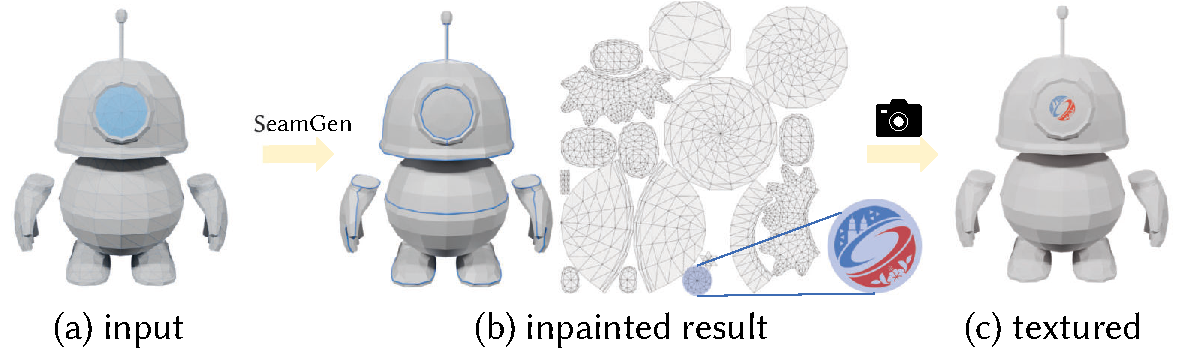
\includegraphics[width=\columnwidth]{figures/user_guide_vis.pdf}
    \caption{
    \textbf{User-guided seam generation via conditional inpainting.}
    (a) The user marks a seam-free region (blue) on the eye area of the mesh, specifying that this region should remain free of cuts.
    (b) Our method completes the remaining seam layout under this constraint and unwraps the mesh into a UV atlas.
    (c) The resulting seam-free eye region provides a clean, continuous surface for texture placement. We insert the SIGGRAPH Asia logo into the corresponding UV region and render the textured result.
    }
    \vspace{-4mm}
    \label{fig:user_guide_vis}
\end{figure}
\subsection{Additional Qualitative Results}
\label{sec:additional_results}

We further demonstrate two practical properties of \methodname{} in production-oriented UV workflows.
First, \methodname{} can preserves structural symmetry when generating seam layouts for symmetric objects. 
As shown in Fig.~\ref{fig:sym}, the generated seams are likely to be placed on corresponding symmetric parts, producing UV islands with compatible shapes after repacking. 
This makes it possible to reuse the same UV space across symmetric regions, improving texture-space utilization and providing a convenient basis for downstream UV-space texture generation and editing. 
We further demonstrate this benefit by generating image textures on the repacked UV layouts using GPT-Image-2~\cite{openai2026gptimage2}.
Second, we evaluate \methodname{} in a component-wise UV unwrapping workflow for complex production assets. 
Although our model is primarily designed for meshes with moderate triangle counts, it can be directly applied to complex models after they are decomposed into semantic components, as commonly done by artists in professional pipelines. 
Fig.~\ref{fig:part} shows an example game asset separated into multiple parts, such as the head, outfit, and accessories. 
Applying \methodname{} to each component produces coherent seam layouts across the full asset, demonstrating its compatibility with practical artist workflows.


\subsection{Conditional Inpainting Applications}
\label{sec:app_inpainting}
We demonstrate the practical utility of conditional seam refinement via the inpainting mechanism introduced in Sec.~\ref{sec:inpainting}.
First, Fig.~\ref{fig:user_guide_vis} demonstrates constraint-guided seam generation. 
Given a user-specified region where seams should be avoided, \methodname{} respects this constraint and completes the remaining cuts into a coherent seam layout. 
This provides simple local control while producing UV layouts suitable for subsequent texture painting.
Second, Fig.~\ref{fig:refinement_vis} shows that the same conditional sampling mechanism can be used for automatic self-refinement. 
When a sampled seam layout produces overlapping UV triangles, \methodname{} locally repairs the problematic region either by adding seams inside the overlapping island or by resampling its boundary together with neighboring islands. 
This corrects many invalid layouts without discarding the entire sample or training an additional repair model. 
Quantitatively, the single-sample predicted overlap rate is reduced from 26.5\% to 3.5\%, demonstrating improved atlas validity.
The detailed refinement procedure is provided in the supplementary material.
% Second, the same mechanism can be used for automatic self-refinement. When a sampled layout produces overlapping UV triangles after parameterization, we fix the reliable parts of the layout and resample only a local region around the problematic island. As illustrated in Fig.~\ref{fig:refinement_vis}, this can be performed either by introducing additional seams inside the overlapping island or by jointly re-sampling the island boundary together with its neighboring islands. This allows the model to correct many invalid samples without discarding the entire layout or training a separate repair model. Quantitatively, this self-refinement procedure reduces the predicted overlap rate from 26.5\% to 3.5\%, demonstrating its effectiveness in improving atlas validity. The concrete refinement procedure and local region selection strategy are provided in the supplementary material.



\begin{figure}[t]
    \centering
    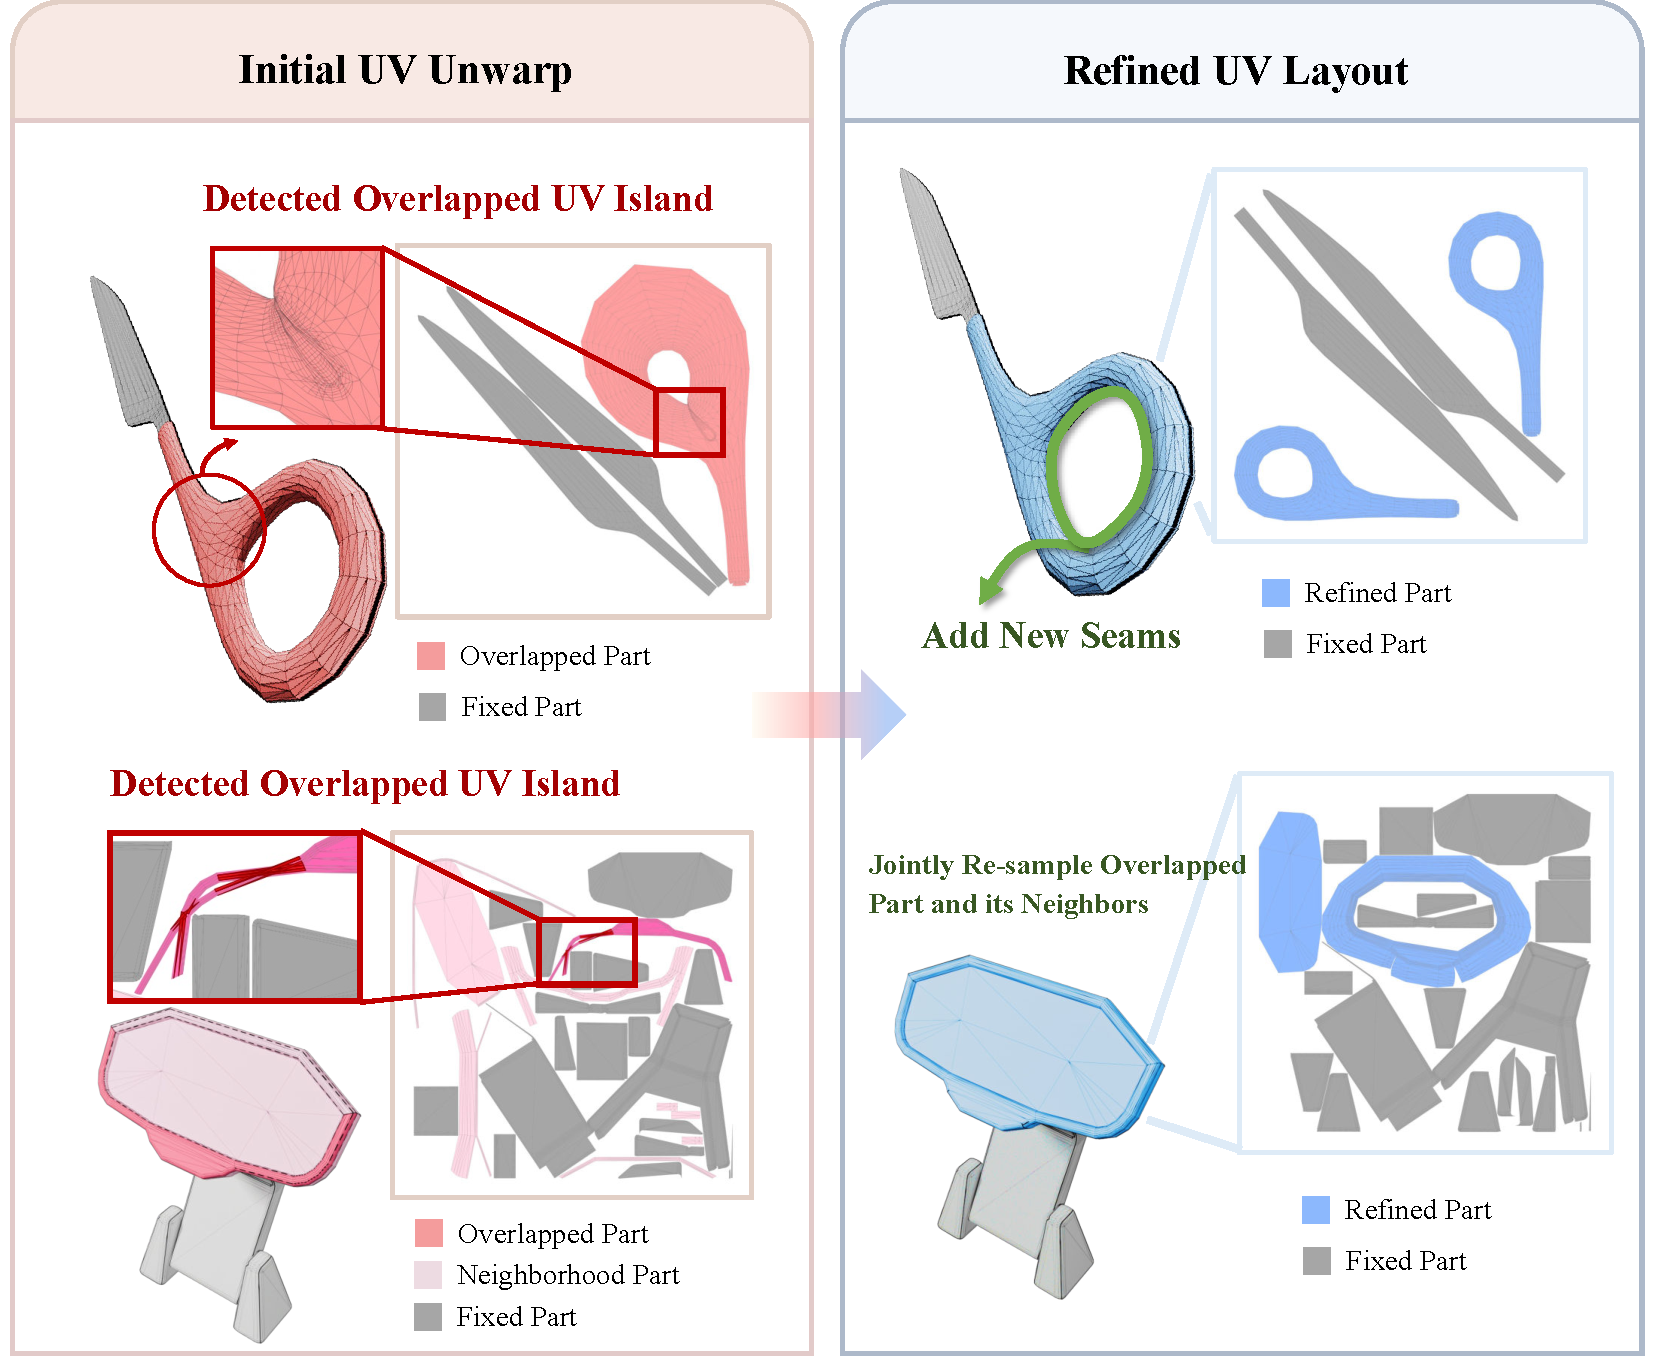
\includegraphics[width=0.99\columnwidth]{figures/uv_refinement.pdf}
    \vspace{-1mm}
    \caption{
    \textbf{Self-refinement via conditional seam inpainting.}
    % Left: initial seam layouts with overlapping UV islands (red).
    % Top: interior-only refinement adds a new seam inside the problematic island.
    % Bottom: boundary-aware refinement jointly resamples the overlapping island and its neighboring islands (yellow).
    % Right: refined, overlap-free UV islands are shown in blue, with newly added seams highlighted in red on the mesh.
    Left: initial layouts with detected overlapping UV islands (red) and their neighborhood (pink). Right: refined, overlap-free UV islands (blue) with updated seam. Top: interior refinement adds new seams (green) within the problematic island. Bottom: boundary-aware refinement jointly resamples the overlapping island and its neighbors. 
    }
    \vspace{-2mm}
    \label{fig:refinement_vis}
\end{figure}

% We evaluate both the architectural design of our Mesh Transformer backbone and the effect of inference-time self-refinement. For the backbone, we consider two variants: \emph{w/o Global Attn}, which removes all global self-attention modules and propagates information purely through the local stream along the mesh connectivity; and \emph{Naive GraphConv}, which keeps the global self-attention stream but replaces the local attention module with a vanilla graph convolution. Since some form of local message passing along mesh edges is structurally necessary for injecting topology, we replace this stream rather than removing it entirely. For a fair comparison, all backbone variants, including the full model, are trained from scratch on the same dataset for 100 epochs under identical optimization settings.

% In addition, we report an inference-time variant, \emph{self-refined}, which uses the full trained model with automatic self-refinement and directly evaluates the initially sampled seam layout. Comparing this variant with the full pipeline measures the effectiveness of the conditional inpainting mechanism when used for automatic overlap correction. All variants are evaluated on the same 200-mesh validation set used in Sec.~\ref{sec:quantitative}. As the evaluation metric, we report the predicted overlap rate, defined as the fraction of meshes whose generated seam layouts produce overlapping UV triangles after flattening; lower is better.

% We ablate both the architectural design of our Mesh Transformer backbone and the inference-time overlap resolution procedure introduced in Sec.~\ref{sec:refinement}. Specifically, we consider three variants: \emph{w/o inpainting}, which uses the full trained model but disables the progressive overlap resolution at inference and reports the single-shot generation result; \emph{w/o Global Attn}, which removes all global self-attention modules and propagates information purely through the local stream along the mesh connectivity; and \emph{Naive GraphConv}, which keeps the global self-attention stream but replaces the local attention module with a vanilla graph convolution. Since some form of local message passing along mesh edges is structurally necessary for injecting topology, we replace this stream rather than removing it entirely. For a fair comparison, all backbone variants, including the full model, are trained from scratch on the same dataset for 100 epochs under identical optimization settings. The \emph{w/o inpainting} variant shares the trained full-model weights and differs only at inference time. All variants are evaluated on the same 200-mesh validation set used in Sec.~\ref{sec:quantitative}. As the evaluation metric, we report the predicted overlap rate, defined as the fraction of meshes whose generated seam layouts produce overlapping UV triangles after flattening; lower is better.

% Our progressive overlap-resolution strategy substantially improves the validity of generated seam layouts at inference time. Starting from the base model predictions, the proposed two-stage inpainting procedure reduces the overlap rate to 3.5\%, successfully resolving roughly seven out of eight overlapping cases without any additional training. This shows that most invalid samples do not need to be discarded and regenerated from scratch, but can instead be corrected through localized conditional seam refinement. For a clean architectural comparison, we next focus on the backbone variants without inpainting. Removing the global self-attention stream increases the overlap rate to 48.1\%, indicating that long-range communication is important for producing globally coherent seam layouts. Replacing the local attention stream with a naive graph convolution is even more detrimental, raising the overlap rate to 72.6\%. This suggests that expressive local modeling is the most critical component of the backbone. Unlike local attention, a simple graph convolution cannot adaptively emphasize geometrically salient neighboring edges, and therefore captures fine-scale seam cues much less effectively. Overall, these ablations show that the local and global streams play complementary roles: the local stream anchors seams to geometrically meaningful boundaries, while the global stream promotes consistency across distant mesh regions. Built on top of this backbone, our progressive inpainting strategy further improves robustness by repairing the remaining overlap failures at inference time, yielding the lowest final overlap rate among all variants.
% We ablate both the architectural design of our Mesh Transformer backbone and the inference-time overlap resolution procedure introduced in Sec.~\ref{sec:refinement}. We consider three variants: w/o inpainting, which uses the full trained model but disables the progressive overlap resolution at inference and reports the single-shot generation result; w/o Global Attn, which removes all global self-attention modules and propagates information purely along the mesh connectivity through the local stream; and Naive GraphConv, which keeps the global self-attention stream but replaces the local attention module with a vanilla graph convolution, since some form of local message passing along the mesh edges is structurally necessary to inject topology, we substitute rather than remove this stream. All variants, including the full model, are trained from scratch on the same dataset for 100 epochs under identical optimization settings for a fair comparison; the w/o inpainting  variant shares the trained full-model weights and differs only at inference. All variants are evaluated on the 200-mesh validation set used in Sec.~\ref{sec:quantitative}. We measure structural quality via the \textbf{predicted overlap rate}, defined as the fraction of meshes whose generated seam layout produces overlapping triangles after flattening; lower is better.





% Disabling the progressive overlap resolution at inference (\emph{w/o inpainting}) raises the predicted overlap rate from 3.5\% to 26.5\%, since every failure must be salvaged by redrawing a fresh noise sample rather than locally repaired; the two-stage inpainting procedure recovers roughly seven out of eight of these failures without any additional training. Among the backbone ablations, which likewise skip inpainting for a clean architectural comparison, removing the global self-attention stream raises the predicted overlap rate from 26.5\% to 48.1\%: without long-range communication, seams initiated on one side of the mesh fail to coordinate with those on the opposite side, so UV islands more often wrap around the surface and self-intersect after flattening. Replacing the local attention with a naive graph convolution is even more damaging---the predicted overlap rate jumps to 72.6\%---indicating that an expressive local stream is in fact the most critical component of the backbone. The simpler graph convolution cannot adaptively weight neighboring edges by their geometric salience, so the network loses the fine-grained cues (dihedral angles, local curvature, proximity to sharp creases) that anchor seams to natural boundaries, and the resulting cuts drift away from geometrically meaningful edges; the global stream alone is unable to compensate for this loss of local precision. Only the full model, in which local attention and global self-attention interleave in every block and the progressive inpainting salvages residual overlap, attains the lowest overlap rate, confirming that the two backbone streams are complementary and that the inference-time inpainting further strengthens the pipeline end-to-end.

% Our progressive overlap-resolution strategy is highly effective at repairing invalid seam layouts at inference time. Starting from the base model predictions, the proposed two-stage inpainting procedure reduces the overlap rate to 3.5\%, successfully resolving roughly seven out of eight overlapping cases without any additional training. This shows that most failures do not require discarding the entire sample; instead, they can be corrected through localized conditional seam refinement, making the overall pipeline substantially more reliable in practice.

% For a clean comparison of backbone architectures, we evaluate the following model variants without inpainting. Removing the global self-attention stream increases the overlap rate to 48.1\%, indicating that long-range communication is important for producing globally coherent seam layouts. Without global context, seam decisions made in one region cannot coordinate well with distant regions on the mesh, so the resulting UV islands are more likely to wrap around the surface inconsistently and self-overlap after flattening.

% Replacing the local attention stream with a naive graph convolution is even more detrimental, leading to an overlap rate of 72.6\%. This suggests that expressive local modeling is the most critical component of the backbone. Unlike local attention, a simple graph convolution cannot adaptively emphasize geometrically salient neighboring edges, and therefore captures fine-scale seam cues much less effectively. As a result, the model becomes less sensitive to dihedral angles, local curvature, and proximity to sharp creases, causing seams to drift away from natural cut boundaries. In this case, global communication alone is insufficient to compensate for the loss of local geometric precision.

% Overall, these ablations show that the local and global streams play complementary roles: the local attention stream anchors seams to geometrically meaningful boundaries, while the global self-attention stream promotes consistency across distant mesh regions. Built on top of this backbone, our progressive inpainting strategy further improves robustness by repairing the remaining overlap failures at inference time, yielding the lowest final overlap rate among all variants.

\section{Conclusion, Limitations, and Future Work}
We presented \methodname{}, a flow-matching generative framework that learns the distribution of artist-authored UV seam layouts directly on the mesh graph. By designing a Mesh Transformer backbone that interleaves local message passing along mesh edges with global self-attention over all vertices, \methodname{} captures both fine-grained geometric cues and long-range context required for production-quality seam placement. A training-free inpainting procedure inherited from the flow matching formulation enables both user-guided seam generation and iterative resolution of overlapping UV islands with a single pretrained model, without heuristic post-processing or auxiliary training objectives. Experiments show that \methodname{} produces seam layouts whose seam-structure and UV-island statistics closely match the ground-truth distribution, outperforming distortion-based and semantic-proxy baselines across quantitative metrics, qualitative comparisons, and user studies.

Despite these results, several limitations remain. 
First, evaluating whether a generated seam distribution closely matches the ground truth remains challenging. 
There is still no direct and widely accepted metric for measuring distribution-level alignment with artist-authored seam layouts. 
Although we use UV-layout statistics, VLM-based evaluation, and a user study as complementary evidence, designing better objective metrics for artist-aligned seam assessment remains an important direction for future work.
Second, \methodname{} may occasionally produce invalid UV atlases. 
In the worst case, a small number of problematic islands may require local fallback to traditional unwrapping methods.
% Conditional inpainting can repair many local failures, but does not guarantee overlap-free or distortion-optimal results.
Finally, our current implementation may exceed GPU memory for meshes with more than roughly 30K faces. 
Future hierarchical graph designs could improve scalability to high-resolution assets.

% Despite these results, several limitations remain. 
% First, evaluating the perceptual quality of seam layouts remains challenging. 
% While our structural seam and island statistics quantify several measurable properties of the generated layouts, they only serve as indirect proxies for alignment with artist-authored conventions. 
% In particular, there is still no widely accepted numerical metric that directly measures whether a seam layout matches artist preferences in terms of semantic placement, visual unobtrusiveness, and practical editability. 
% We therefore complement our quantitative evaluation with a user study, and we believe that designing better objective metrics for artist-aligned seam layout assessment is an important direction for future work.
% Second, as a generative model, \methodname{} samples from a learned distribution, and occasional failure cases may still occur when the sampled seams deviate from artist-authored conventions or lead to invalid parameterizations. 
% Although conditional inpainting can correct many local failures, it does not provide a formal guarantee of overlap-free or distortion-optimal UV maps. 
% Finally, scalability to very high-resolution meshes remains limited. 
% In our current implementation, meshes with more than roughly 30K faces can exceed GPU memory, limiting direct application to very high-resolution production assets. 
% Future work could explore hierarchical, patch-based, or coarse-to-fine graph representations to reduce memory consumption and enable seam generation on larger meshes.

%%%%%%%%% REFERENCES
{
    \small
    \bibliographystyle{ieeenat_fullname}
    \bibliography{main}
}

\begin{figure*}[p]
    \centering
    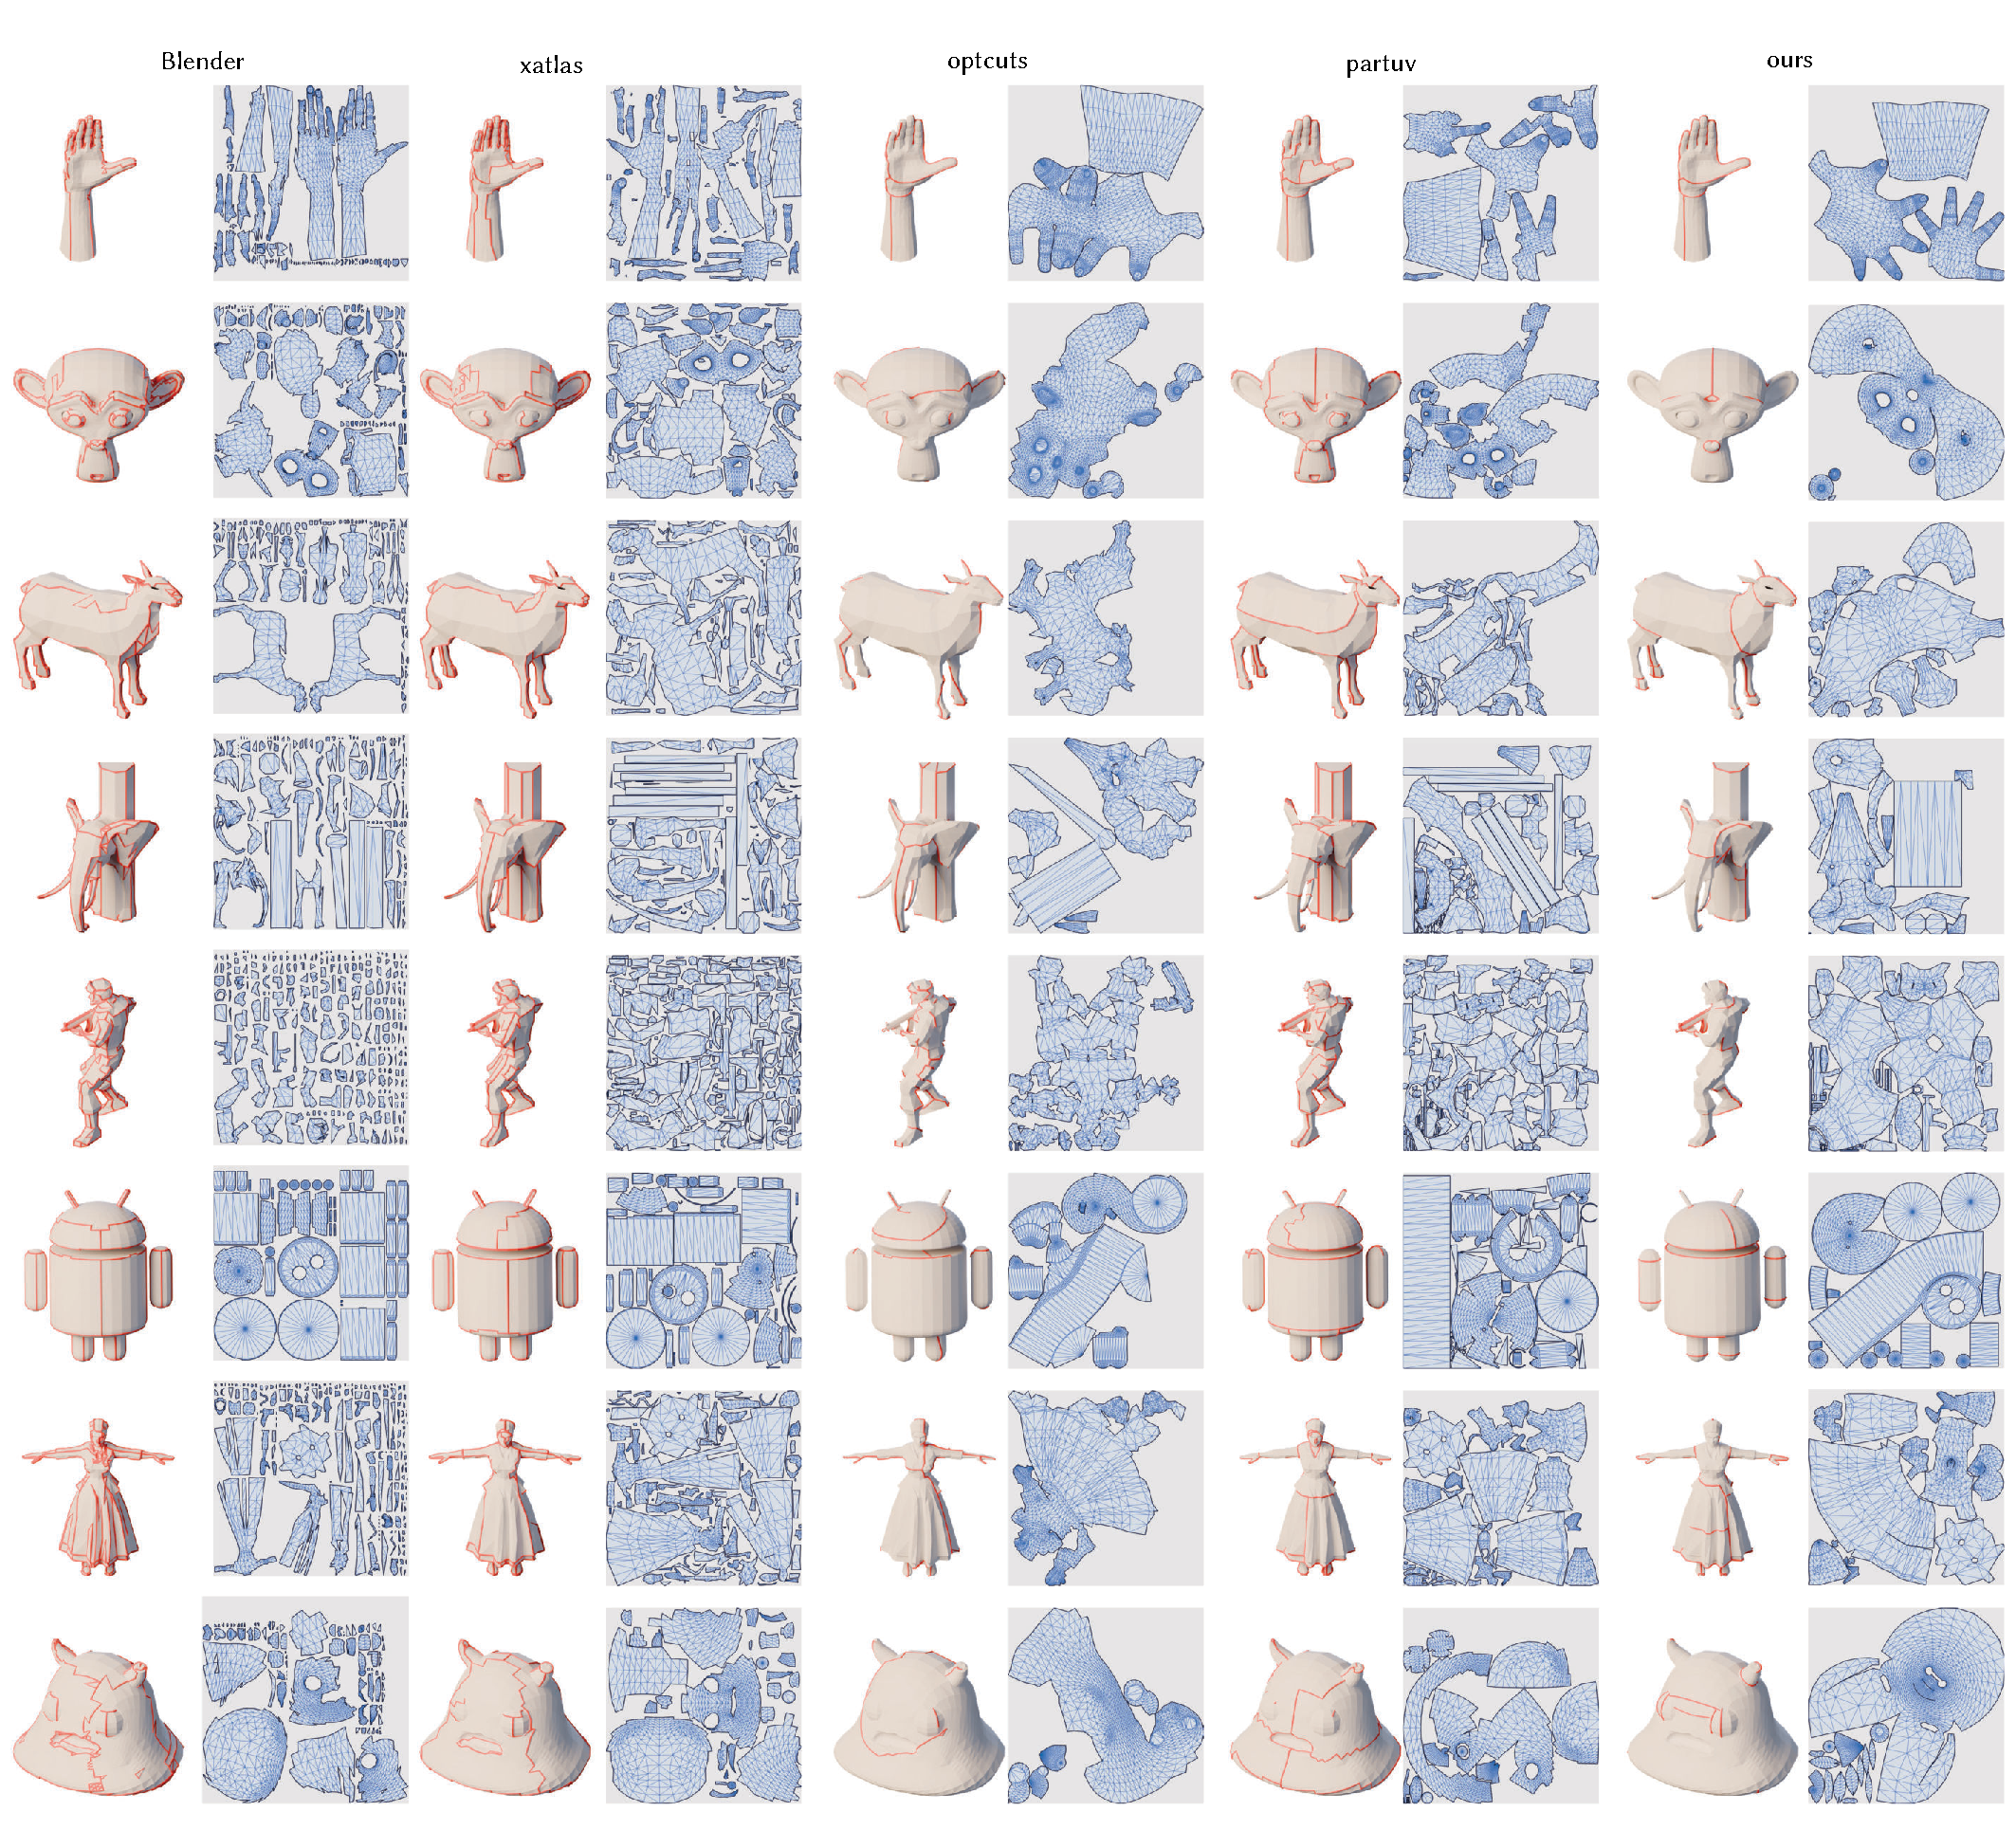
\includegraphics[width=\linewidth]{figures/qualitative.pdf}
    \caption{\textbf{Qualitative comparison} of UV unwrapping results on representative meshes. From left to right, we show the results of Blender~\cite{blender}, xatlas~\cite{young2019xatlas}, OptCuts~\cite{li2018optcuts}, PartUV~\cite{wang2025partuv}, and \methodname{} (ours). For each method, we visualize the seam layout on the mesh and its corresponding UV map; seam edges are highlighted in red. Compared with the baselines, \methodname{} produces more complete and coherent seam layouts, yielding UV atlases that more closely resemble artist-authored references.}
    \label{fig:qualitative}
\end{figure*}

\begin{figure*}[p]
    \centering
    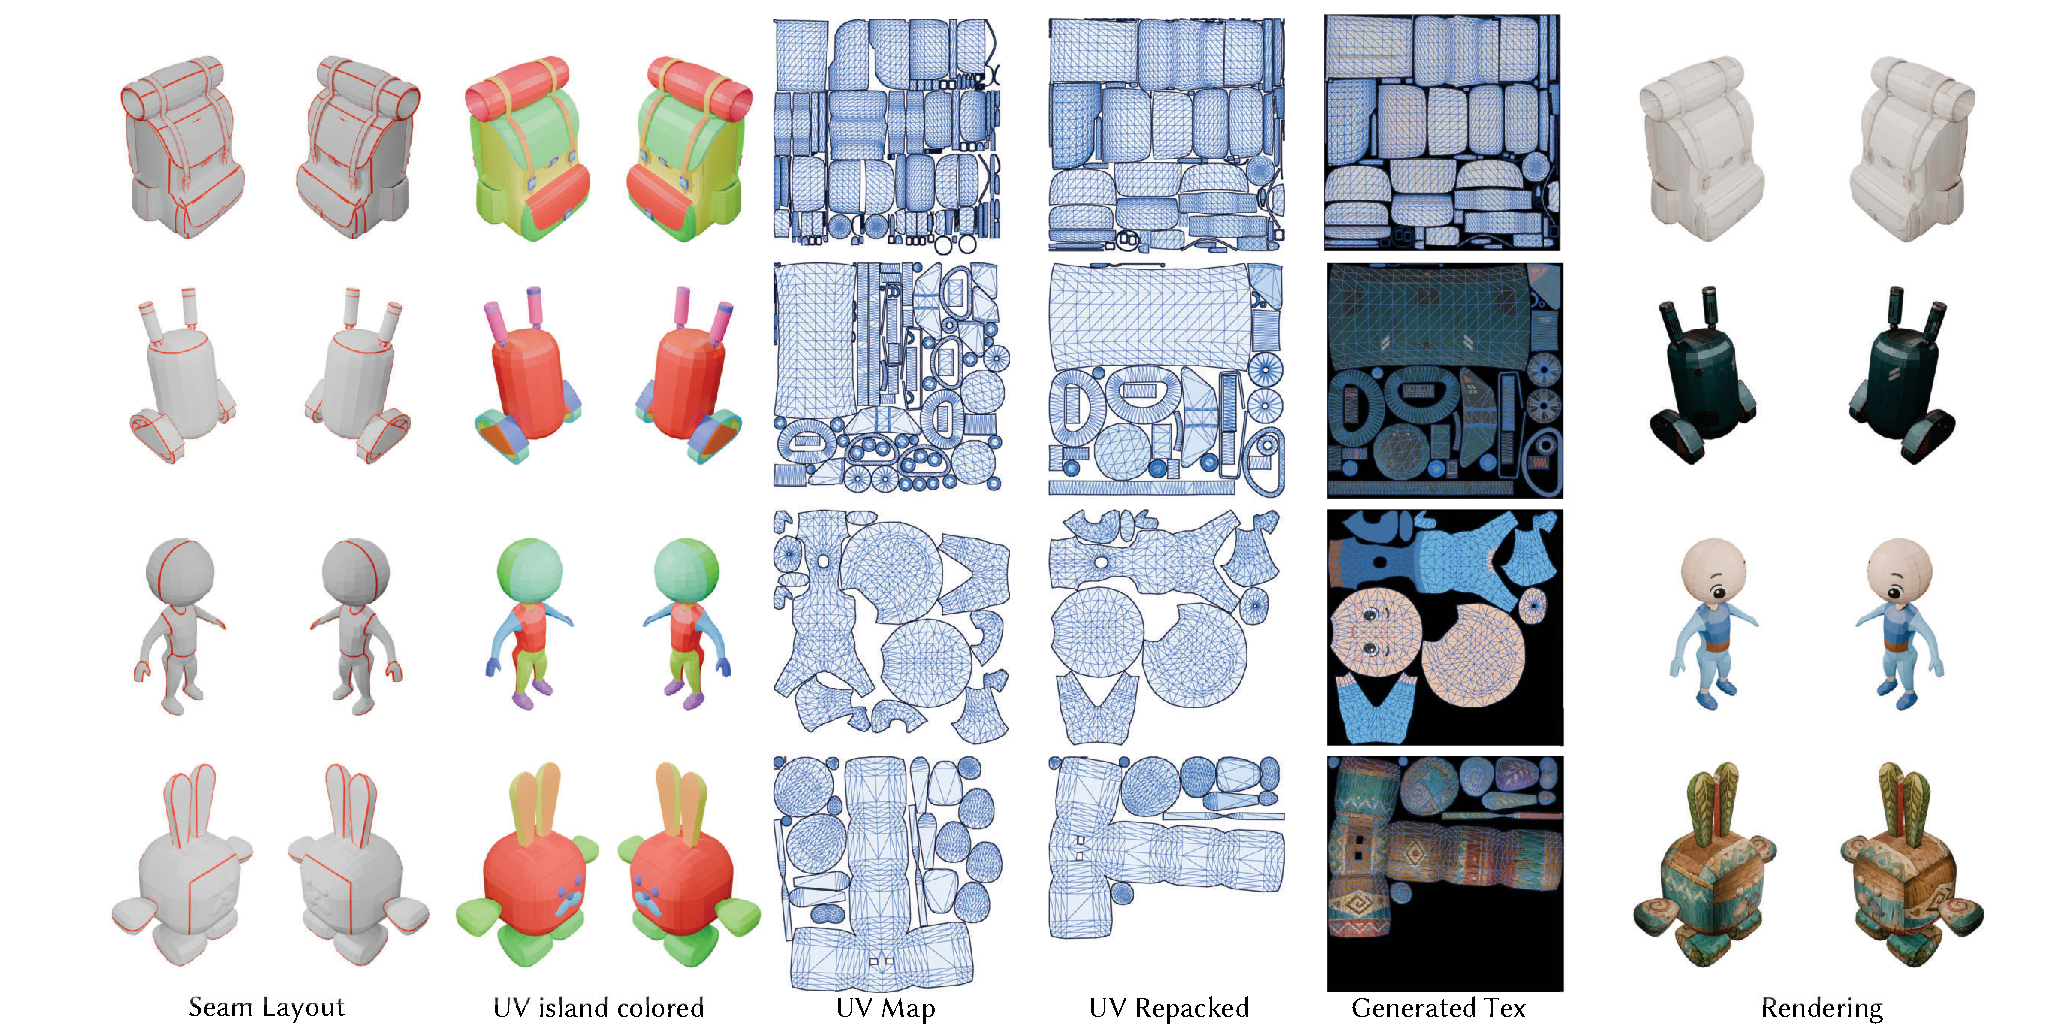
\includegraphics[width=0.96\linewidth]{figures/sym.pdf}
    \caption{\textbf{Qualitative results of symmetric seam layouts and downstream texturing.} We show that our method inherently respects the structural symmetry of input meshes during seam generation, enabling symmetric parts to share the same UV space after repacking. This significantly enhances texture utilization, providing a superior foundation for downstream UV-space texture generation and editing.}
    \label{fig:sym}
\end{figure*}

\begin{figure*}[p]
    \centering
    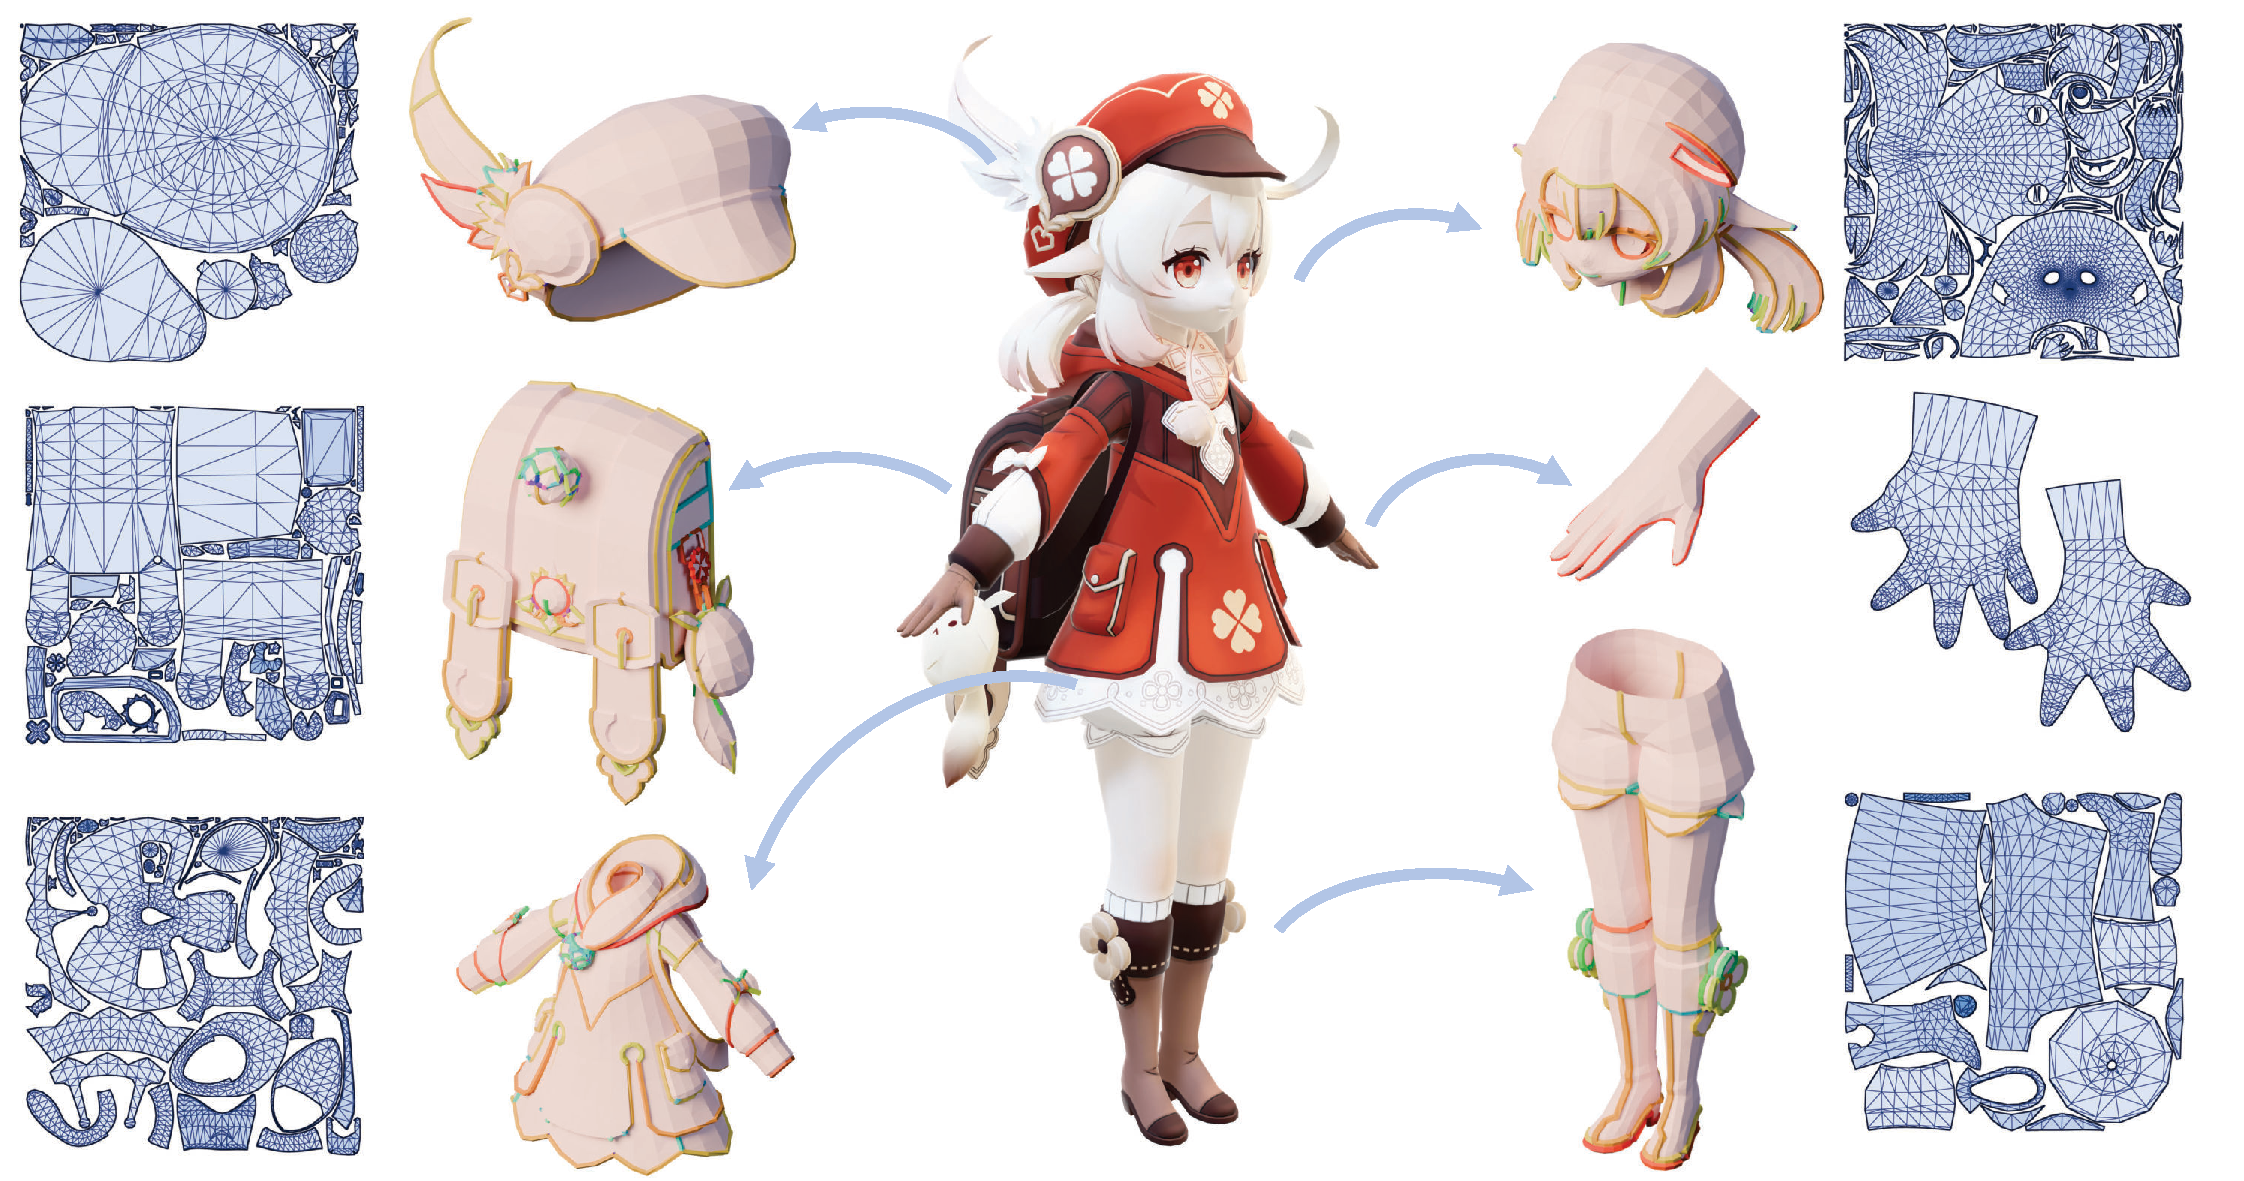
\includegraphics[width=0.99\linewidth]{figures/part.pdf}
    \caption{\textbf{Component-wise UV Seam Generation integrated with professional art workflows.} Although our model is primarily designed for meshes with moderate triangle counts, it perfectly adapts to professional production pipelines. In practice, artists typically decompose complex characters into multiple semantic parts (e.g., head, outfit, accessories) for UV unwrapping. Our method seamlessly integrates into this workflow, ensuring high-quality seam placement across all individual components.}
    \label{fig:part}
\end{figure*}

\end{document}
